% Paquets généraux
\documentclass[a4paper,12pt,titlepage,twoside]{article}
\usepackage[T1]{fontenc}
\usepackage[utf8]{inputenc}
\usepackage[french]{babel}
\usepackage{subcaption}
\addto\captionsfrench{%
  \renewcommand{\tablename}{Tableau}%
}
\usepackage[gen]{eurosym}
%\usepackage[dvips]{graphicx}
\usepackage{minted}
\usepackage{fancyhdr}
\usepackage{pdfpages} 
\usepackage{multido}
\usepackage{hyperref}
\usepackage{textcomp}
\usepackage{schemabloc}
%\usepackage[bitstream-charter]{mathdesign}
\usepackage{array}
\newcolumntype{P}[1]{>{\centering\arraybackslash}p{#1}}
\usepackage[shortlabels]{enumitem}
\usepackage[framemethod=TikZ]{mdframed}

\newcommand{\id}{71}
\newcommand{\nom}{Théorie des mécanismes}
\newcommand{\sequence}{04}
\newcommand{\nomsequence}{Liaisons entre les solides}
\newcommand{\num}{02}
\newcommand{\type}{KH}
\newcommand{\descrip}{Liaisons équivalentes, hyperstatisme, liaisons en série et en parallèle, théorie des graphes}
\newcommand{\competences}{B2-12: Proposer une modélisation des liaisons avec leurs caractéristiques géométriques. \\ &  B2-13: Proposer un modèle cinématique paramétré à partir d'un système réel, d'une maquette numérique ou d'u \\ &  B2-17: Simplifier un modèle de mécanisme. \\ &  B2-18: Modifier un modèle pour le rendre isostatique. \\ &  C1-04: Proposer une démarche permettant d'obtenir une loi entrée-sortie géométrique.  \\ &  C2-05: Caractériser le mouvement d'un repère par rapport à un autre repère. \\ &  C2-06: Déterminer les relations entre les grandeurs géométriques ou cinématiques. }
\newcommand{\nbcomp}{7}
\newcommand{\systemes}{}
\newcommand{\systemesnum}{}
\newcommand{\systemessansaccent}{}
\newcommand{\ilot}{2}
\newcommand{\ilotstr}{02}
\newcommand{\dossierilot}{\detokenize{Ilot_02 }}

%\usepackage{style}
\usepackage{bodegraph}
\usepackage{rpcinematik}
\usepackage[locale = FR]{siunitx}
\usepackage{caption}
\newcommand{\institute}{Lycée Dorian}

\usepackage{listings}
\usepackage{fancyvrb}
\usepackage{color}
\usepackage{xcolor}
\usepackage{colortbl}
\usepackage{helvet}
\usepackage[frenchmath]{newtxsf} % for sans serif symbols
\renewcommand{\familydefault}{\sfdefault}
%\usepackage{amsfonts}
%\usepackage{amsmath}
%\usepackage{lmodern}
\usepackage{mathastext}
%\usepackage{xspace}
\usepackage{varioref}
\usepackage{tabularx}
%\usepackage{floatflt}
\usepackage{graphics}
\usepackage{wrapfig}
\usepackage{textcomp}
\usepackage{tikz,tkz-tab}
\usepackage[european resistor, european voltage, european current]{circuitikz}
\usepackage{wrapfig}
\usepackage{gensymb}
\usepackage[percent]{overpic}
\usetikzlibrary{babel}
\usepackage{ifthen}
\usepackage{cancel}
\usepackage{etoolbox}
\usepackage{multirow}
%\usepackage{boxedminipage}
\definecolor{gris25}{gray}{0.75}
\definecolor{bleu}{RGB}{18,33,98}
\definecolor{bleuf}{RGB}{42,94,171}
\definecolor{bleuc}{RGB}{231,239,247}
\definecolor{bleum}{RGB}{160,195,226}
\definecolor{rougef}{RGB}{185,18,27}
\definecolor{rougec}{RGB}{255,188,204}%255,230,231
\definecolor{vertf}{RGB}{103,126,82}
\definecolor{vertc}{RGB}{220,255,191}
\definecolor{forestgreen}{rgb}{0.13,0.54,0.13}
\definecolor{blcr}{rgb}{0.59,0.69,0.84}
\definecolor{blfr}{rgb}{0.32,0.51,0.75}
\definecolor{orfr}{rgb}{0.90,0.42,0.15}
\definecolor{orcr}{rgb}{0.90,0.65,0.50}
\definecolor{orangef}{rgb}{0.659,0.269,0.072}
\definecolor{orange}{rgb}{0.58,0.35,0.063}
\definecolor{orangec}{rgb}{0.43,0.32,0.25}
\definecolor{rcorrect}{rgb}{0.6,0,0}
\definecolor{sequence}{rgb}{0.75,0.75,0.75}
\definecolor{competences}{rgb}{0.61,0.73,0.35}
\definecolor{rose}{HTML}{ff00ff}
\definecolor{grisf}{HTML}{222222}
\definecolor{grisc}{HTML}{636363}
\definecolor{normal}{HTML}{4087c4}
\definecolor{info}{HTML}{5bc0de}
\definecolor{success}{RGB}{92,184,92}
\definecolor{warning}{RGB}{240,173,78}
\definecolor{danger}{RGB}{217,83,79}
\hypersetup{                    % parametrage des hyperliens
    colorlinks=true,                % colorise les liens
    breaklinks=true,                % permet les retours à la ligne pour les liens trop longs
    urlcolor= blfr,                 % couleur des hyperliens
    linkcolor= orange,                % couleur des liens internes aux documents (index, figures, tableaux, equations,...)
    citecolor= forestgreen                % couleur des liens vers les references bibliographiques
    }

\newcolumntype{M}[1]{>{\centering\arraybackslash}m{#1}}
\definecolor{codegreen}{rgb}{0,0.6,0}
\definecolor{codegray}{rgb}{0.5,0.5,0.5}
\definecolor{codepurple}{rgb}{0.58,0,0.82}
\definecolor{backcolour}{rgb}{0.95,0.95,0.92}

\lstdefinestyle{mystyle}{
    backgroundcolor=\color{backcolour},   
    commentstyle=\color{codegreen},
    keywordstyle=\color{magenta},
    numberstyle=\tiny\color{codegray},
    stringstyle=\color{codepurple},
    basicstyle=\ttfamily\footnotesize,
    breakatwhitespace=false,         
    breaklines=true,                 
    captionpos=b,                    
    keepspaces=true,                 
    numbers=left,                    
    numbersep=5pt,                  
    showspaces=false,                
    showstringspaces=false,
    showtabs=false,                  
    tabsize=2
}

\lstset{style=mystyle}

% Mise en page
\pagestyle{fancy}

\setlength{\hoffset}{-18pt}
\setlength{\oddsidemargin}{0pt} 	% Marge gauche sur pages impaire2s
\setlength{\evensidemargin}{0pt} 	% Marge gauche sur pages paires
\setlength{\marginparwidth}{00pt} 	% Largeur de note dans la marge
\setlength{\headwidth}{481pt} 	 	% Largeur de la zone de tête (17cm)
\setlength{\textwidth}{481pt} 	 	% Largeu\textbf{r de la zone de texte (17cm)
\setlength{\voffset}{-18pt} 		% Bon pour DOS
\setlength{\marginparsep}{7pt}	 	% Séparation de la marge
\setlength{\topmargin}{-30pt} 		% Pas de marge en haut
\setlength{\headheight}{55pt} 		% Haut de page
\setlength{\headsep}{20pt} 		% Entre le haut de page et le texte
\setlength{\footskip}{30pt} 		% Bas de\textbf{ page + séparation
\setlength{\textheight}{700pt} 		% Hauteur de l'icone zone de texte (25cm)
\setlength\fboxrule{1 pt}
\renewcommand{\baselinestretch}{1}
\setcounter{tocdepth}{1}
\newcommand{\cadre}[2]
{\fbox{
  \begin{minipage}{#1\linewidth}
   \begin{center}
    #2\\
   \end{center}
  \end{minipage}
 }
}

\newcommand{\repon}[1]
{
~\ \\
\begin{tabular}{|m{\linewidth}|}
 \hline
\multido{}{#1}{\\ \hline}
\end{tabular}
}


\newcommand{\objectif}[1]{
\mdfsetup{%
frametitle={%
\tikz[baseline=(current bounding box.east),outer sep=0pt]
\node[anchor=east,rectangle,fill=bleum]
{\strut Objectif~};}}
\mdfsetup{innertopmargin=10pt,linecolor=bleum,%
linewidth=2pt,topline=true,%
frametitleaboveskip=\dimexpr-\ht\strutbox\relax
}
\begin{mdframed}[]\relax%
#1
\end{mdframed}}


\newcounter{num_quest} \setcounter{num_quest}{0}
\newcounter{num_rep} \setcounter{num_rep}{0}
\newcounter{num_cor} \setcounter{num_cor}{0}

\newcommand{\feuilleDR}[1]{
	\begin{tikzpicture}
		\draw[gray!30](0,0)grid[step=0.5cm](\linewidth,#1);
	\end{tikzpicture}
}

%\newcommand{\question}[1]{\refstepcounter{num_quest}\par
%~\ \\ \parbox[t][][t]{0.15\linewidth}{\textbf{Question \arabic{num_quest}}}\parbox[t][][t]{0.85\linewidth}{#1\label{q\the\value{num_quest}}}\par
%}

\newcommand{\question}[1]{\refstepcounter{num_quest}\par
~\ \\ \textbf{Question \arabic{num_quest} : }#1\label{q\the\value{num_quest}}\par
}

\newcommand{\posetafigure}[3]{
\begin{figure}[ht!]
 \begin{center}
  \includegraphics[width=#2\linewidth]{img/#1}
 \end{center}
 \caption{\label{#1} #3}
\end{figure}}

\newcommand{\goforum}{
\begin{figure}

\end{figure}
\begin{center}
 
\includegraphics[width=0.7\linewidth]{../../../img/go_forum}
\end{center}
\label{go_forum}
\caption{J'pète les plombs}
\end{figure}}

\newcommand{\reponse}[4][1]
{\noindent
\parbox{\textwidth}{
\rule{\linewidth}{.5pt}\\
\textbf{Question\ifthenelse{#1>1}{s}{} \multido{}{#1}{%
\refstepcounter{num_rep}\ref{q\the\value{num_rep}} }:} ~\ \\
\ifdef{\public}{#3 \ifthenelse{#2>0}{~\ \\ 	\feuilleDR{#2}}}{#4}
}}

\newcommand{\cor}
{\refstepcounter{num_cor}
\noindent
\rule{\linewidth}{.5pt}
\textbf{Question \arabic{num_cor}:} \\
}

\newcommand{\finsujet}
{
    \begin{center}
    \Large{FIN}
    \end{center}

    \cleardoublepage

    \ifdef{\public}{\pagestyle{docreponse}}{\pagestyle{correction}}

    \ifdef{\public}{
        \begin{tikzpicture} 
            \draw (0,0) rectangle (2,2);
            \draw (0,0) -- (2,2);
            \draw (1.5,0.5) node {\large 20};
            \draw (2.5,0) rectangle (16,2);
            \draw (4.5,1.7) node {\large Commentaires:};
        \end{tikzpicture}
    }
    ~\ \\
}


%\newcommand{\repcarre}[2]
%{
%~\ \\
%\begin{tikzpicture}
%\draw [fill=white] (0,0) rectangle +(\linewidth,#1);
%\node[align=left] at (1.1,#2-0.3) {\textbf{Question #1:}};
%\end{tikzpicture}
%}

\newcommand{\titre}[1]
{\begin{center}
\cadre{0.8}{\huge #1} 
\end{center}
}


%Définition des torseurs :
\newcommand{\torseur}[2]{\left\{\mathcal{#1}_{#2} \right\}}
\newcommand{\torseurh}[3]{\left\{\genfrac{}{}{0pt}{0}{#1}{#2}\right\}_{#3}}
\newcommand{\torseurv}[8]{\left\{
\begin{matrix}
#1 & #4 \\ #2 & #5 \\ #3 &#6
\end{matrix}
\right\}_{{#7},{#8}}}

%Définition des torseurs :
%\newcommand{\torseur}[2]{\left \{\mbox{\relsize{2}{$\mathcal {#1}$}\relsize{-2}}\phantom{}_{\mbox{\scriptsize $#2$}} \right \}}
%\newcommand{\torseurh}[3]{\left\{\genfrac{}{}{0pt}{0}{#1}{#2}\right\}_{#3}}
%\newcommand{\torseurv}[8]{
%\left\{\begin{array}{@{}c|c@{}} #1 & #4 \\ #2 & #5 \\ #3 & #6 \end{array} \right\}_{#7,#8}
%}
\newcommand{\derivee}[2]{\left.\dfrac{\d #1}{\d t}\right|_{#2}}
\newcommand{\tripleint}{\int\!\!\!\!\!\int\!\!\!\!\!\int}

% Notation cinématique et statique
\newcommand{\cinematique}[2]{\mbox{#1}/\mbox{#2}}
\newcommand{\statique}[2]{\mbox{#1}\rightarrow\mbox{#2}}
\newcommand{\moment}[3]{\vv {#1}_{\scriptsize{#3}}(#2)}
\newcommand{\resultante}[2]{\vv {#1}_{\scriptsize{#2}}}


%Commande de base
\newcommand{\jo}{\left(j\omega\right)} % j \omega dans l'analyse fréquentielle
\newcommand{\tl}{\xrightarrow{\mathcal{L}}} % transformée de laplace sur fleche
\newcommand{\tli}{\xrightarrow{\mathcal{L}^{-1}}} % transformée inverse de laplace sur fleche
\renewcommand{\d}[1][]{\mathrm{d#1}}
\newcommand{\dd}[1][]{\mathrm{d#1}}
\newcommand{\vect}[2]{{#1}\wedge{#2}}
\newcommand{\base}[3]{(\vec #1,\vec #2,\vec #3)}
\newcommand{\vectbase}[4]{{\vphantom{\left| \begin{matrix}
#1\\#2\\#3 \end{matrix} \right|}}_{#4}{\left| \begin{matrix}
#1\\#2\\#3 \end{matrix} \right.}}
%Pour avoir les paragraphes sous la forme I, II, III
\renewcommand{\thesection}{\Roman{section}}
\setcounter{secnumdepth}{3}
\renewcommand{\Frlabelitemii}{$\bullet$}

% En tête et pied de page
\lhead{\nom}
\rhead{
\includegraphics[width=2cm]{../../../img/logo}}
\lfoot{\auteurun,\ \auteurdeux}
\cfoot{Page \thepage}

\fancypagestyle{docreponse}{%
  \fancyhf{}
  \fancyhead[LO]{NOM Prénom: .............................}
  \rhead{
\includegraphics[width=2cm]{../../../img/logo}\hspace{2pt}}
  \ifdef{\auteurdeux}{\lfoot{\auteurun,\ \auteurdeux}}{\lfoot{\auteurun}}
  \rfoot{\nom}
  \lfoot{Document réponse}
  \cfoot{Page \thepage}
   }

\fancypagestyle{correction}{%
  \fancyhf{}
  \lhead{\colorbox{danger}{\begin{minipage}{0.65\paperwidth} \textcolor{white}{\textbf{Correction}} \end{minipage}} }
  \rhead{
\includegraphics[width=2cm]{../../../img/logo}}
  \lfoot{Renaud Costadoat, Françoise Puig}
  \rfoot{\colorbox{danger}{\begin{minipage}{0.4\paperwidth} \begin{flushright}\textcolor{white}{\textbf{Correction}}\end{flushright} \end{minipage}} }}

\fancypagestyle{correctioninfo}{%
  \fancyhf{}
  \lhead{\colorbox{danger}{\begin{minipage}{0.65\paperwidth} \textcolor{white}{\textbf{Correction}} \end{minipage}} }
  \rhead{
\includegraphics[width=2cm]{../../../img/logo}}
  \lfoot{Renaud Costadoat, Juliette Genzmer}
  \rfoot{\colorbox{danger}{\begin{minipage}{0.6\paperwidth} \begin{flushright}\textcolor{white}{\textbf{Correction}}\end{flushright} \end{minipage}} }}

\renewcommand{\footrulewidth}{0.4pt}

\usepackage{eso-pic}
\newcommand{\BackgroundPic}{%
\put(0,0){%
\parbox[b][\paperheight]{\paperwidth}{%
\vfill
\begin{center}
\hspace{0.5cm}\vspace{0.5cm}
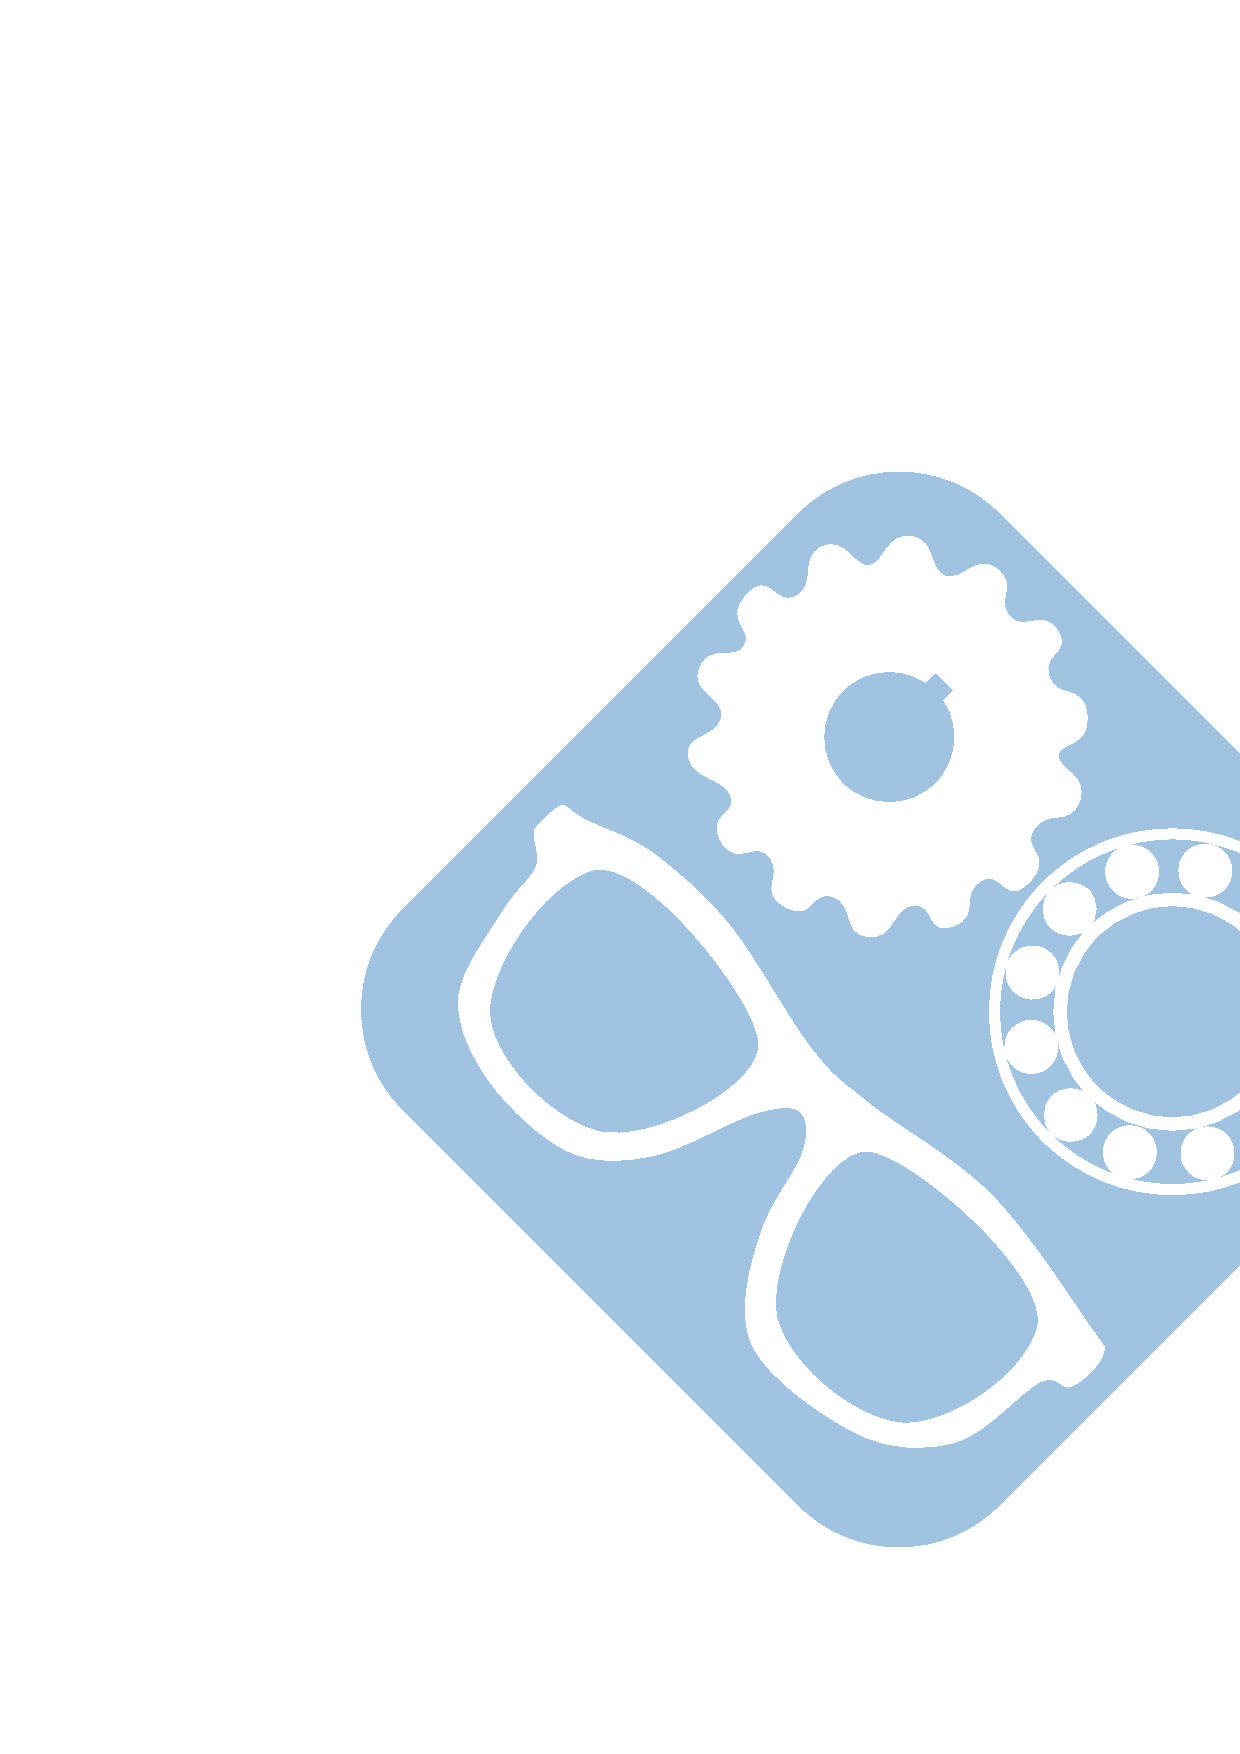
\includegraphics[width=\paperwidth,height=\paperheight,%
keepaspectratio]{../../../img/fond3}%
\end{center}
\vfill
}}}

\newcommand{\BackgroundPicdeux}{%
\put(25,-30){%
\parbox[b][\paperheight]{\paperwidth}{%
\vfill
\begin{center}
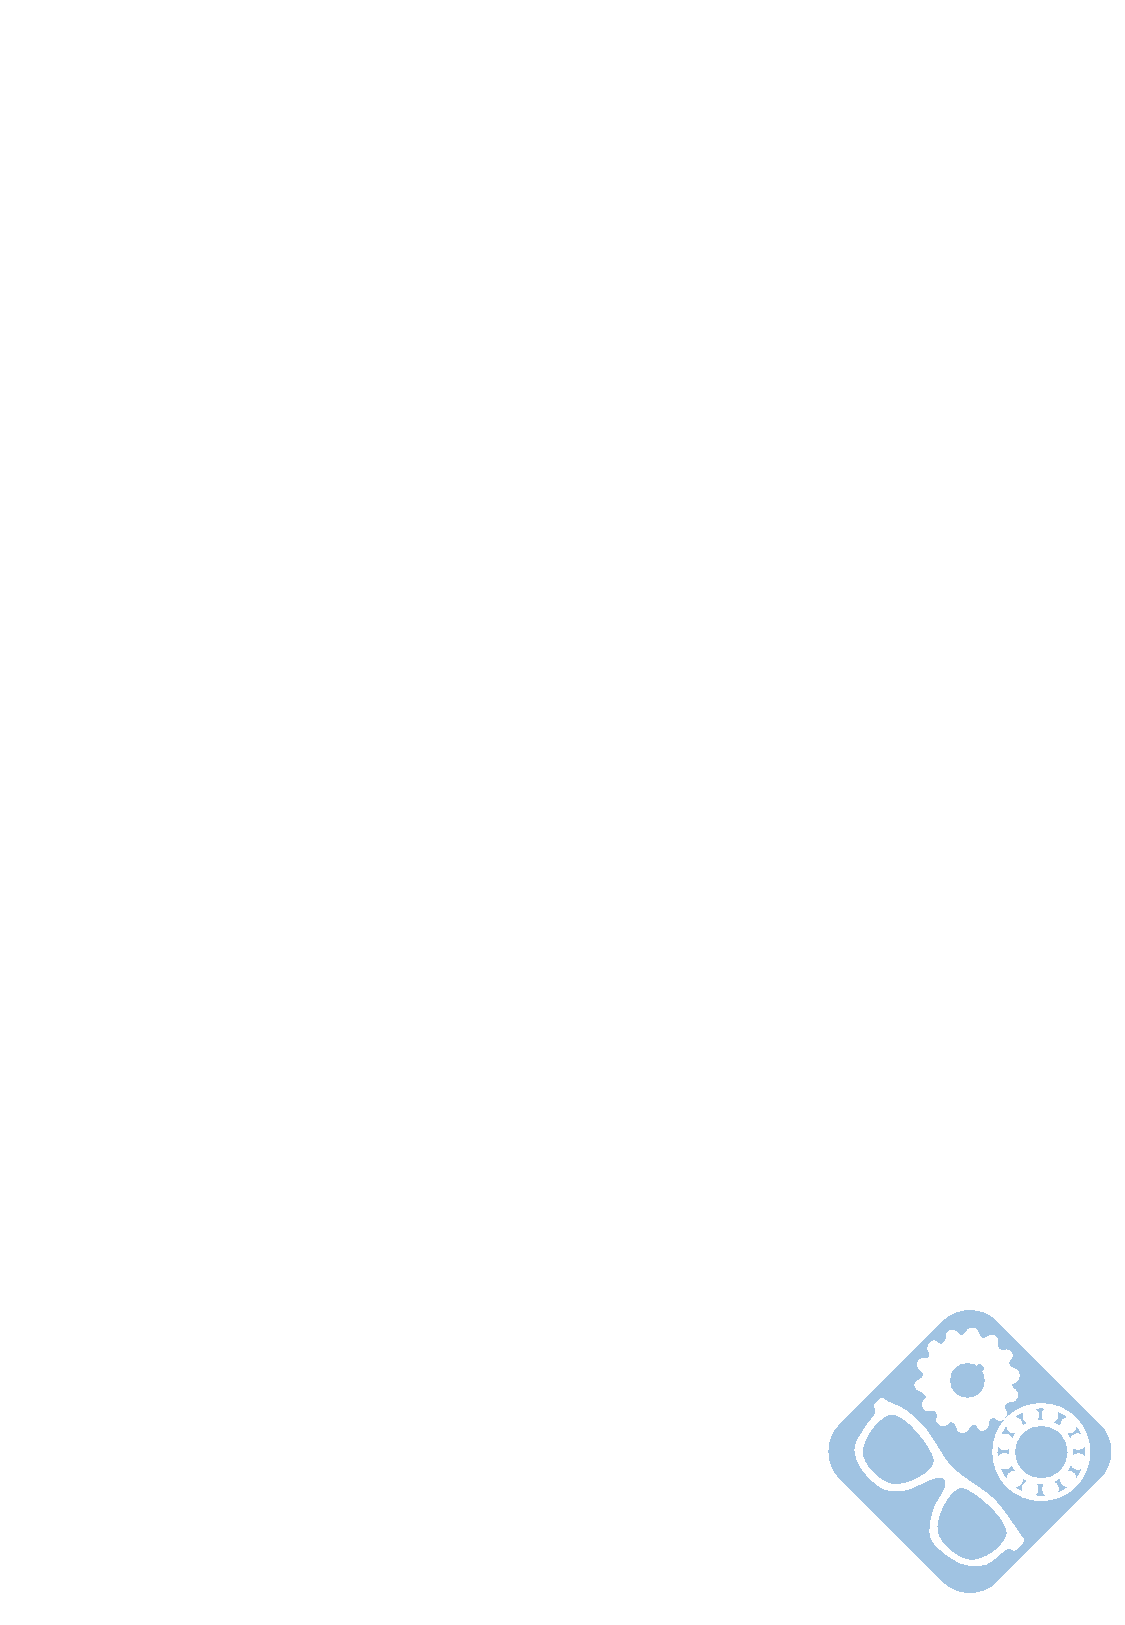
\includegraphics[width=\paperwidth,height=\paperheight,%
keepaspectratio]{../../../img/fond4}%
\end{center}
\vfill
}}}

\begin{document}

\pagestyle{empty}

\AddToShipoutPicture*{\BackgroundPic}


\includegraphics[width=2cm]{../../../img/logo}

\Huge{DS \numero - \sujet}

\vspace{1cm}

\ifdef{\prive}{\begin{center}\colorbox{danger}{\Huge{Avec Correction}}\end{center}}{}

\begin{center}
\centering\huge{PTSI}
\end{center}

\vspace{2cm}


\begin{center}
\centering\Large{\jour}
\end{center}

\vspace{2cm}

\normalsize

\tableofcontents

\newpage

\AddToShipoutPicture{\BackgroundPicdeux}

\pagestyle{fancy}

\begin{center}
\Huge \sujet
\end{center}


\normalsize


\section{Présentation générale (30 min)}

\subsection{Contexte}

L'exosquelette est un appareil qui apporte à un être humain des capacités qu'il ne possède pas ou qu'il a
perdues à cause d'un accident. Ce type d'appareil peut permettre à une personne de soulever des charges
lourdes et diminuer considérablement les efforts à fournir sans la moindre fatigue (figure \ref{img01}). Après avoir revêtu un exosquelette adapté à sa morphologie et à sa taille, l'utilisateur peut faire ses mouvements en bénéficiant d'une grande fluidité.

\begin{figure}[!h]
 \centering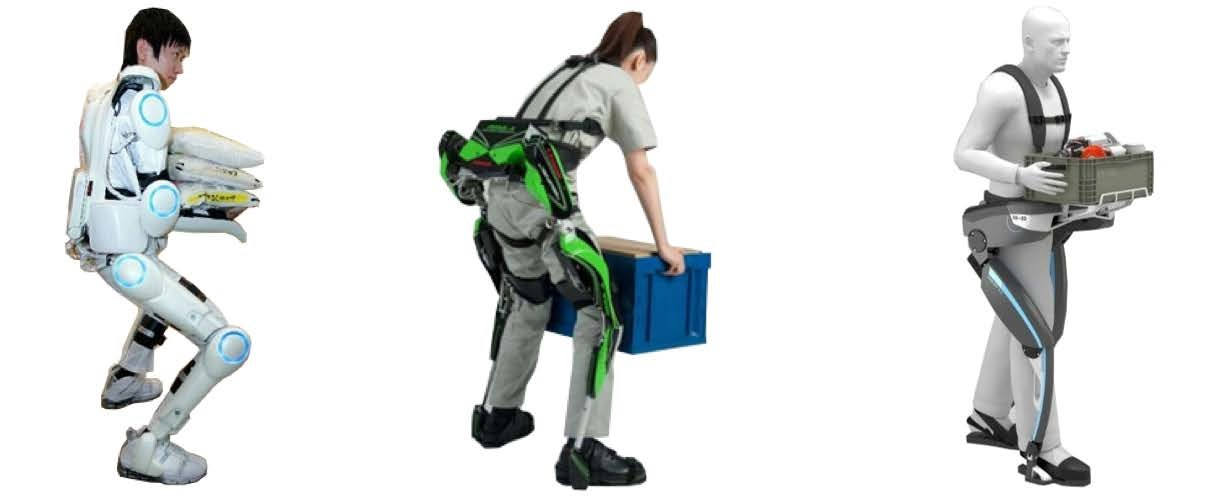
\includegraphics[width=0.9\linewidth]{img/fig01}
 \caption{Maniement de charges}
 \label{img01}
\end{figure}


\subsection{Mise en situation}

L'exosquelette (figure \ref{img02}) est constitué :
\begin{itemize}
 \item d'un support de charge transportée 4,
 \item de deux moteurs de l'articulation de la hanche,
 \item de deux cuisses 2 et 2',
 \item de deux moteurs de genou,
 \item de deux jambes 1 et 1',
 \item de deux articulations de cheville, non motorisées,
 \item de deux pieds 3 et 3'.
\end{itemize}

\begin{figure}[!h]
 \centering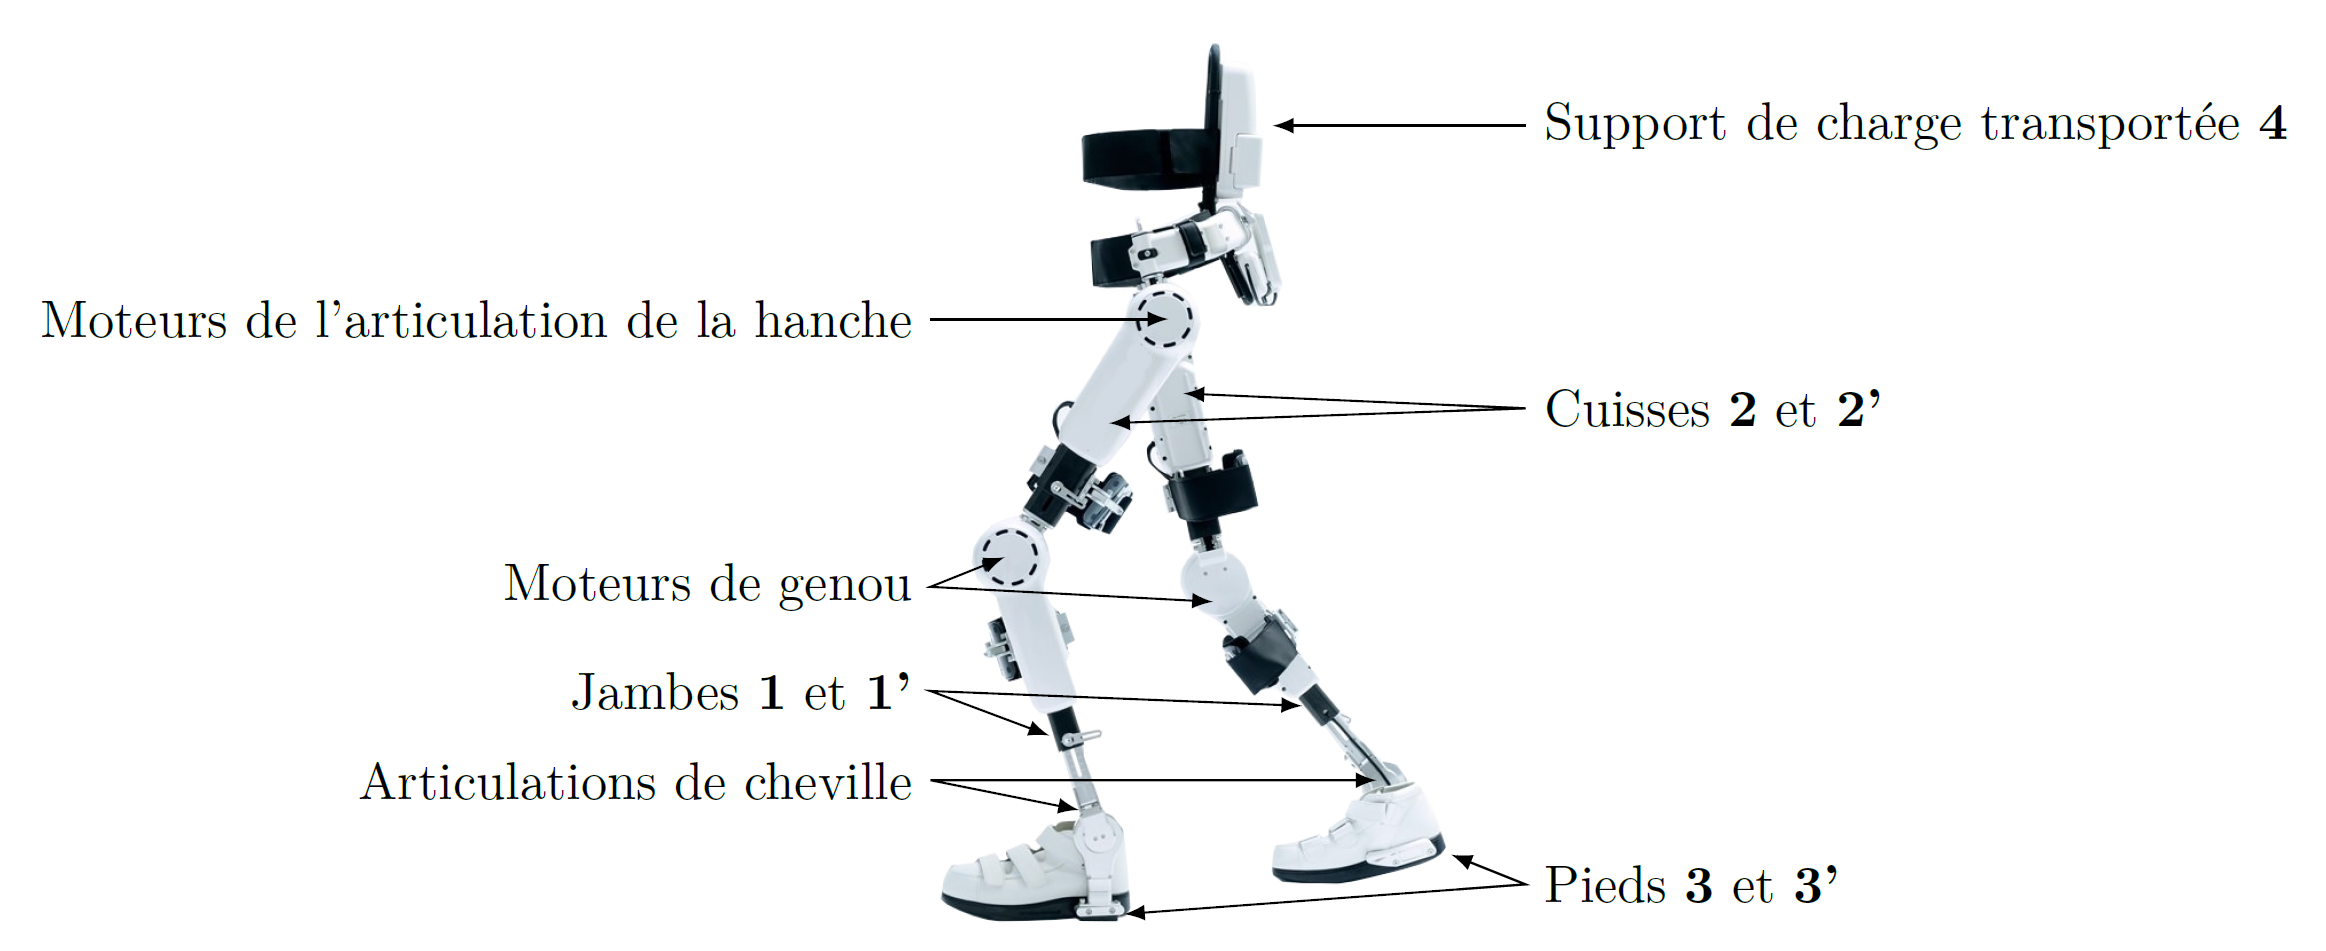
\includegraphics[width=0.9\linewidth]{img/fig02}
 \caption{Constituants de l'exosquelette}
 \label{img02}
\end{figure}

Les actionneurs équipant chaque axe (genoux et hanches) de l'exosquelette sont des moteurs synchrones de
type \og brushless \fg, couplés à des réducteurs de vitesse de type \og Harmonic Drive \fg. Chaque moteur est alimenté par une carte de positionnement incluant un onduleur triphasé, la source d'énergie étant un pack de batteries de tension nominale égale à 36 V. La carte de positionnement exploite les signaux des capteurs à effet Hall intégrés dans le moteur ainsi que ceux d'un codeur incrémental monté sur l'axe moteur, elle comprend trois asservissements :
\begin{itemize}
 \item un asservissement de courant qui correspond à un asservissement de couple,
 \item un asservissement de vitesse avec un correcteur proportionnel et intégral,
 \item un asservissement de position offrant des fonctions d'anticipation de vitesse.
\end{itemize}

Les moteurs au niveau de l'articulation de la hanche permettent de modifier l'inclinaison de la charge afin
d'éviter un basculement autour de son axe de tangage. Une centrale inertielle est utilisée à cet effet. Un modèle multiphysique de l'exosquelette est représenté figure \ref{img03}.

\begin{figure}[!h]
 \centering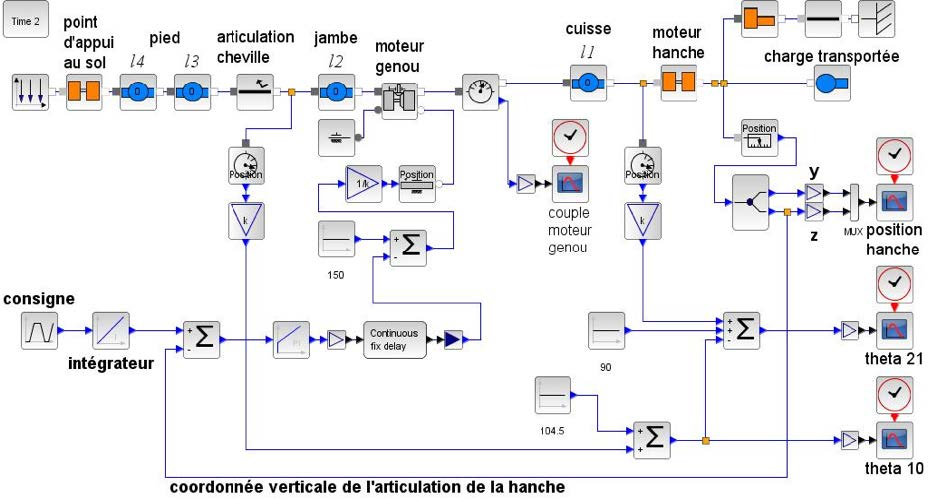
\includegraphics[width=0.9\linewidth]{img/fig03}
 \caption{Modèle multiphysique de l'exosquelette}
 \label{img03}
\end{figure}

Ce sujet se concentre essentiellement sur le dimensionnement et le pilotage des moteurs des genoux.

\subsection{Étude proposée}

La fluidité de marche et la gestion en temps réel des mouvements (marcher à plat ou sur des pentes jusqu'à 10°, monter des marches, se mettre en position accroupie ou assise) sont des éléments fondamentaux qui conditionnent la conception et la réalisation d'un exosquelette. Les solutions technologiques retenues répondent à cet objectif.

Elles ne sont pas toutes abordées dans ce sujet. Quelques-unes de celles retenues pour l'exosquelette sont étudiées pour valider les solutions choisies par les concepteurs vis-à-vis des performances attendues listées par le cahier des charges.

Dans cette optique, il est proposé les quatre études suivantes :
\begin{itemize}
 \item modélisation et validation des constituants associés à l'exigence fonctionnelle \og assurer le mouvement vertical \fg,
 \item validation de l'architecture de la chaine fonctionnelle réalisant l'exigence fonctionnelle \og gérer le mouvement vertical \fg,
 \item conception de la chaine d'information réalisant l'exigence fonctionnelle \og acquérir l'intention de la mise en mouvement \fg,
 \item évolution du produit.
\end{itemize}

\section{Exigence fonctionnelle \og assurer le mouvement vertical \fg}

\paragraph{Objectif}

Proposer un modèle de connaissance des éléments réalisant l'exigence fonctionnelle \og assurer le mouvement vertical \fg\ puis valider les performances attendues listées par le cahier des charges (tableau \ref{tab01}).

\begin{table}[!h]
\begin{tabular}{|l|l|l|}
\hline
Exigences & Critères d'appréciation & Niveau \\
\hline
\multirow{2}{*}{Assurer le mouvement vertical} & Durée du mouvement de la hanche & t = 2 s \\
 & Masse de la charge à soulever par les deux jambes & m$_4$ = 60 kg \\
\hline
\end{tabular}
 \caption{Extrait du cahier des charges associé à l'exigence \og Assurer le mouvement vertical \fg}
 \label{tab01}
\end{table}

\subsection{Élaboration du modèle géométrique direct et du modèle articulaire inverse}

\paragraph{Objectif}

Élaborer la commande du moteur pilotant le genou à partir d'un mouvement défini dans l'espace
opérationnel puis converti dans l'espace articulaire.

L'étude se limite au passage de la position accroupie à la position relevée de l'exosquelette. Lors de ce passage, le point O$_2$ est en mouvement de translation verticale suivant la direction $\overrightarrow{z_0}$ et sa vitesse de déplacement évolue selon une loi trapézoïdale. Un modèle plan de la chaine cinématique ouverte représente la partie inférieure de l'exosquelette en position debout et fléchie (figure \ref{img04}).

\begin{figure}[!h]
 \centering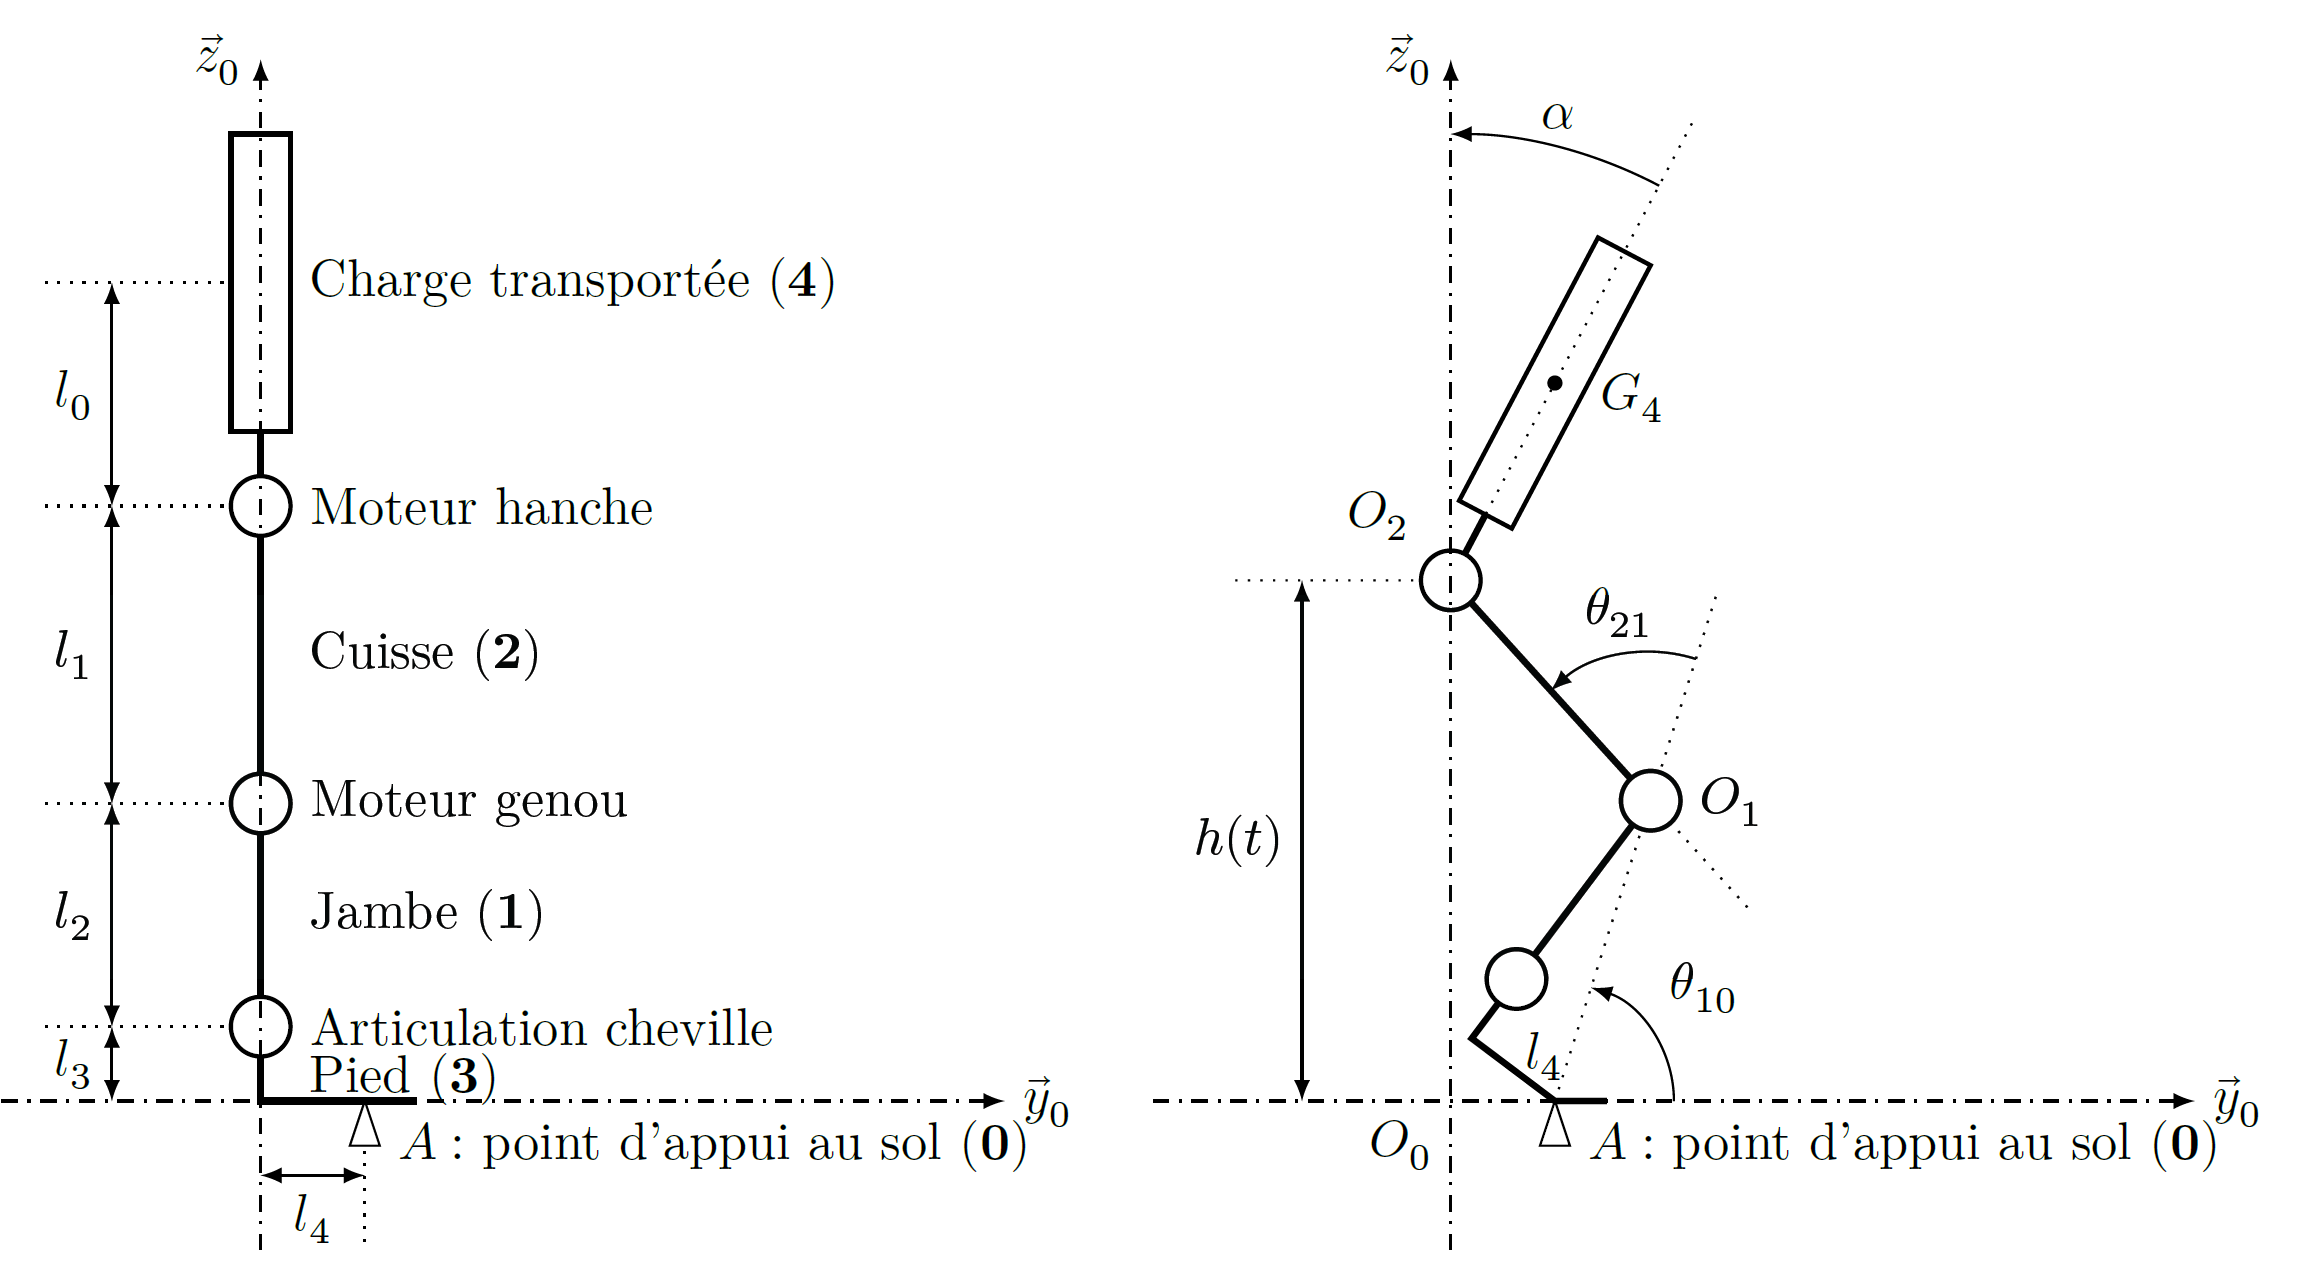
\includegraphics[width=0.9\linewidth]{img/fig04}
 \caption{Modèle d'étude plan position debout et fléchie}
 \label{img04}
\end{figure}

Un modèle d'étude simplifié plan ainsi que l'orientation des repères et le paramétrage angulaire sont proposés
figure \ref{img05}.

Hypothèses:
\begin{itemize}
 \item Le référentiel lié au repère R$_0$(A, $\overrightarrow{x_0}$, $\overrightarrow{y_0}$, $\overrightarrow{z_0}$) est galiléen et est fixe par rapport à la terre,
 \item Le point O$_2$ représentant la hanche se déplace verticalement selon la direction $\overrightarrow{z_0}$,
 \item L'angle $\alpha$ entre la charge transportée et la verticale $\overrightarrow{z_0}$ reste constant,
 \item Le point d'appui A du pied sur le sol est considéré fixe par rapport à la terre,
 \item Lors du mouvement étudié, la jambe (1) reste perpendiculaire au pied (3).
\end{itemize}


Données:
\begin{itemize}
 \item $\theta_{10}$ = ($\overrightarrow{y_0}$, $\overrightarrow{y_1}$) = ($\overrightarrow{z_0}$, $\overrightarrow{z_1}$),
 \item $\theta_{21}$ = ($\overrightarrow{y_1}$, $\overrightarrow{y_2}$) = ($\overrightarrow{z_1}$, $\overrightarrow{z_2}$),
 \item $\alpha$ = constante,
 \item $L = \sqrt{(l_2+l_3)^2+l_4^2}$.
\end{itemize}

\begin{figure}[!h]
 \centering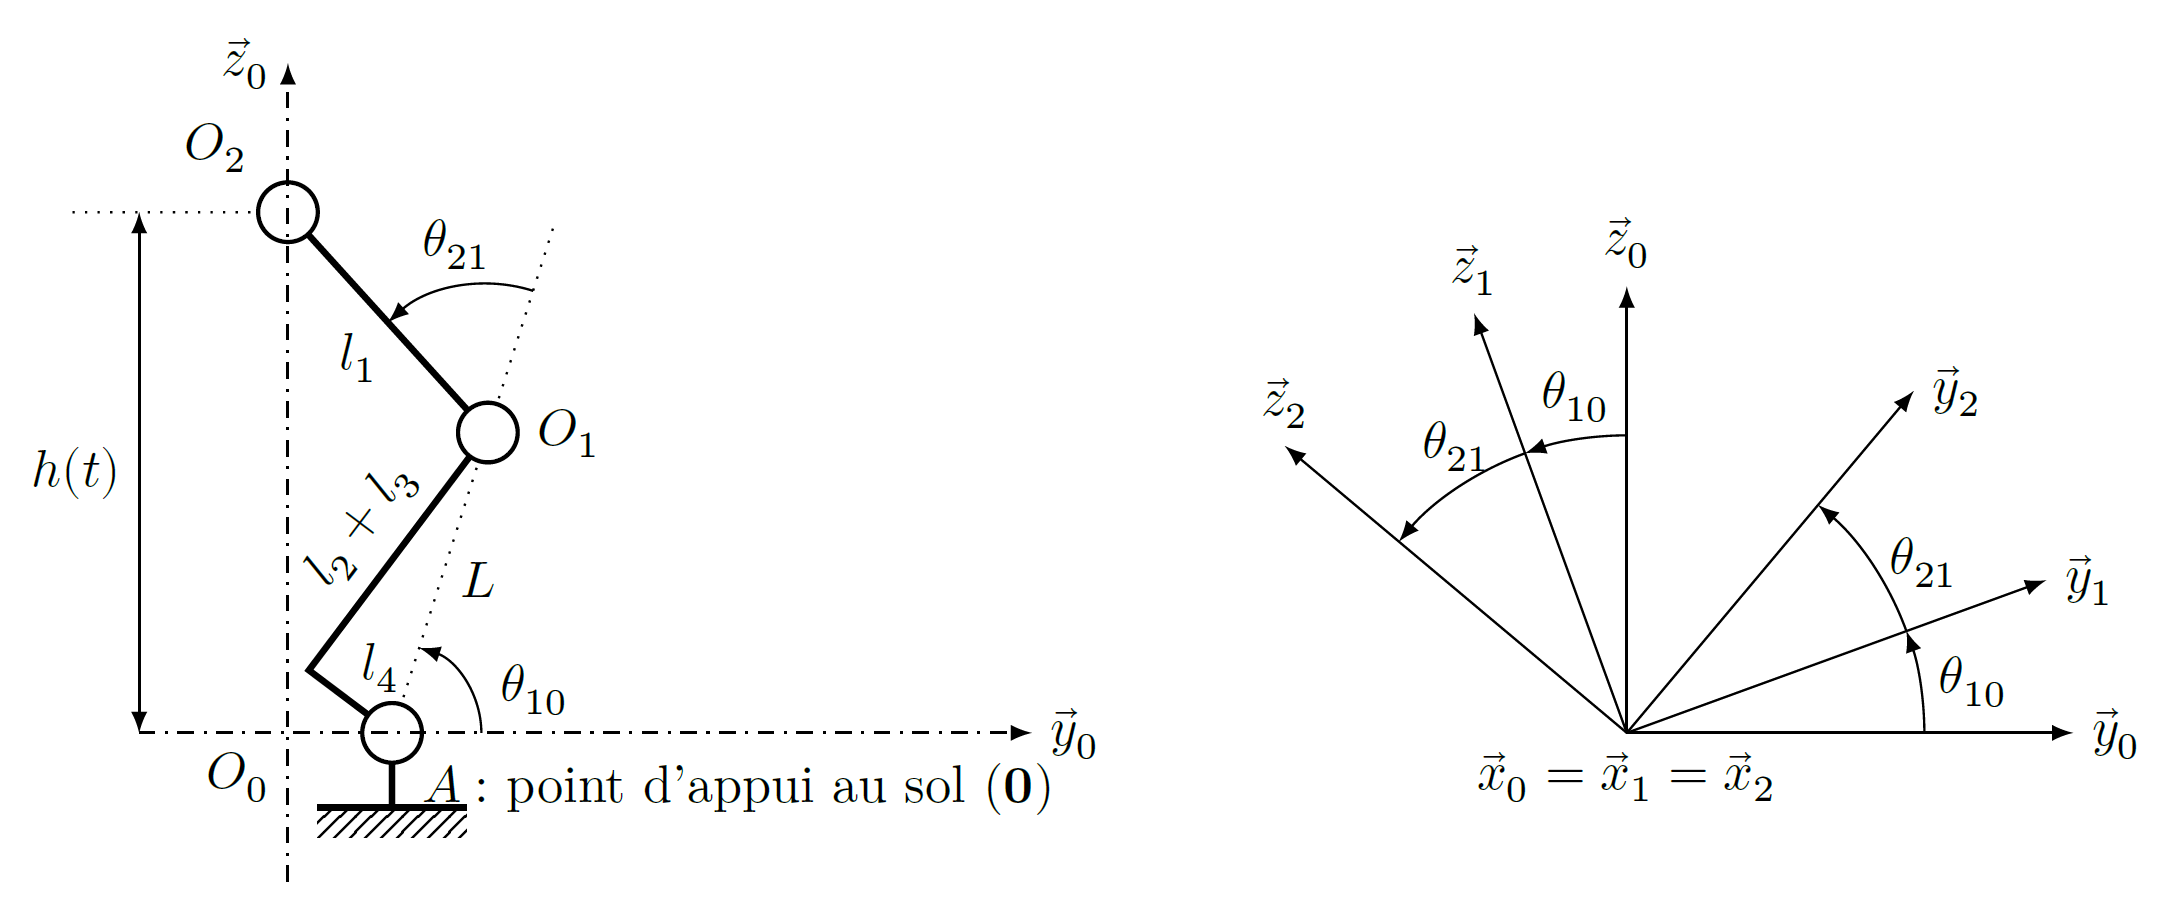
\includegraphics[width=0.9\linewidth]{img/fig05}
 \caption{Modèle simplifié plan et paramétrage angulaire}
 \label{img05}
\end{figure}


\question{En choisissant une fermeture géométrique pertinente, déterminer littéralement les coordonnées opérationnelles $l_4$ et $h(t)$ en fonction des coordonnées articulaires $\theta_{10}$, $\theta_{21}$ et des paramètres dimensionnels $L$ et $l_1$.}

\question{Déterminer le modèle articulaire inverse $\theta_{21}$ en fonction de $l_1$, $l_4$, $L$ et $h(t)$.}

\question{Déterminer le modèle articulaire inverse $\theta_{10}$ en fonction de $l_1$, $l_4$, $L$ et $h(t)$.}

\textbf{Indications:}
\begin{itemize}
 \item Dans un premier temps, il est conseillé de déterminer l'expression de $\theta_{21}$ à partir des deux relations trouvées à la question 1, provenant du modèle géométrique direct, élevées au carré. (On rappelle que cos(a-b)=cos(a).cos(b)+sin(a).sin(b)),
 \item Dans un deuxième temps, pour déterminer l'expression de $\theta_{10}$, utiliser le modèle géométrique direct exprimé préalablement sous la forme:
 \begin{eqnarray}
	l_1.cos(\theta_{10}+\theta_{21}) = -L.cos\theta_{10} - l_4 \\
	l_1.sin(\theta_{10}+\theta_{21}) = h(t) - L.sin\theta_{10}
 \end{eqnarray}
 \item En éliminant $sin(\theta_{10}+\theta_{21})$ et $cos(\theta_{10}+\theta_{21})$, obtenir une équation de la forme $A.cos\theta_{10} + B.sin\theta_{10} = C$,
 \item En normant A et B l'équation devient:
 \begin{eqnarray}
	\frac{A}{\sqrt{A^2+B^2}}.cos\theta_{10}+\frac{B}{\sqrt{A^2+B^2}}.sin\theta_{10}=\frac{C}{\sqrt{A^2+B^2}}
 \end{eqnarray}
 \item En posant $cos \varphi=\frac{A}{\sqrt{A^2+B^2}}$ et $sin \varphi=\frac{B}{\sqrt{A^2+B^2}}$, l'équation devient $cos \varphi.cos \theta_{10}+sin \varphi.sin \theta_{10}=\frac{C}{\sqrt{A^2+B^2}}$ et se ramène à l'écriture:
  \begin{eqnarray}
	cos(\theta_{10}-\varphi)=\frac{C}{\sqrt{A^2+B^2}}
 \end{eqnarray}
 \item Déterminer l'expression de $\theta_{10}$ en fonction de $l_1$, $l_4$, $L$ et $h(t)$.
\end{itemize}	

\question{Effectuer le graphe de liaison du mécanisme de la figure \ref{img04}, on se limitera aux solides 1, 2, 3 et 4.}

\question{Écrire les torseurs cinématiques et des actions mécaniques pour les liaisons de ce système. Utiliser le formalisme suivant:}

\begin{center}
$\left\{V_{i/j}\right\}=\left\{\begin{array}{cc}
\omega_{ijx} & V_{ijx} \\
\omega_{ijy} & V_{ijy} \\
\omega_{ijz} & V_{ijz}
\end{array}\right\}_{O,R_0(\overrightarrow{x_0},\overrightarrow{y_0},\overrightarrow{z_0})}$,
$\left\{T_{i\rightarrow j}\right\}=\left\{\begin{array}{cc}
X_{ij} & L_{ij} \\
Y_{ij} & M_{ij} \\
Z_{ij} & N_{ij}
\end{array}\right\}_{O,R_0(\overrightarrow{x_0},\overrightarrow{y_0},\overrightarrow{z_0})}$
\end{center}

\section{Exigence fonctionnelle \og gérer le mouvement vertical \fg}

\paragraph{Objectif}

Déterminer les réglages de la commande asservie des moteurs genou droit et gauche permettant d'assurer un mouvement vertical ne déséquilibrant pas le porteur de l'exosquelette puis valider les performances attendues listées par le cahier des charges (tableau \ref{tab02}).

La consigne de position des axes moteur genou gauche et droit est représentée figure \ref{img06}. Elle montre des parties qui peuvent être approchées par des constantes, des rampes et des paraboles.

\begin{table}[!h]
\begin{tabular}{|l|l|l|}
\hline
Exigences & Critères d'appréciation & Niveau \\
\hline
\multirow{4}{*}{Gérer le mouvement vertical} & Précision statique de la boucle d'asservissement de position & 
 \\
& erreur de position & < 1\% \\
& erreur de trainage & < 1\% \\
& erreur d'accélération & < 1\% \\
\hline
\end{tabular}
 \caption{Extrait du cahier des charges associé à l'exigence \og Gérer le mouvement vertical \fg}
 \label{tab02}
\end{table}

\begin{figure}[!h]
 \centering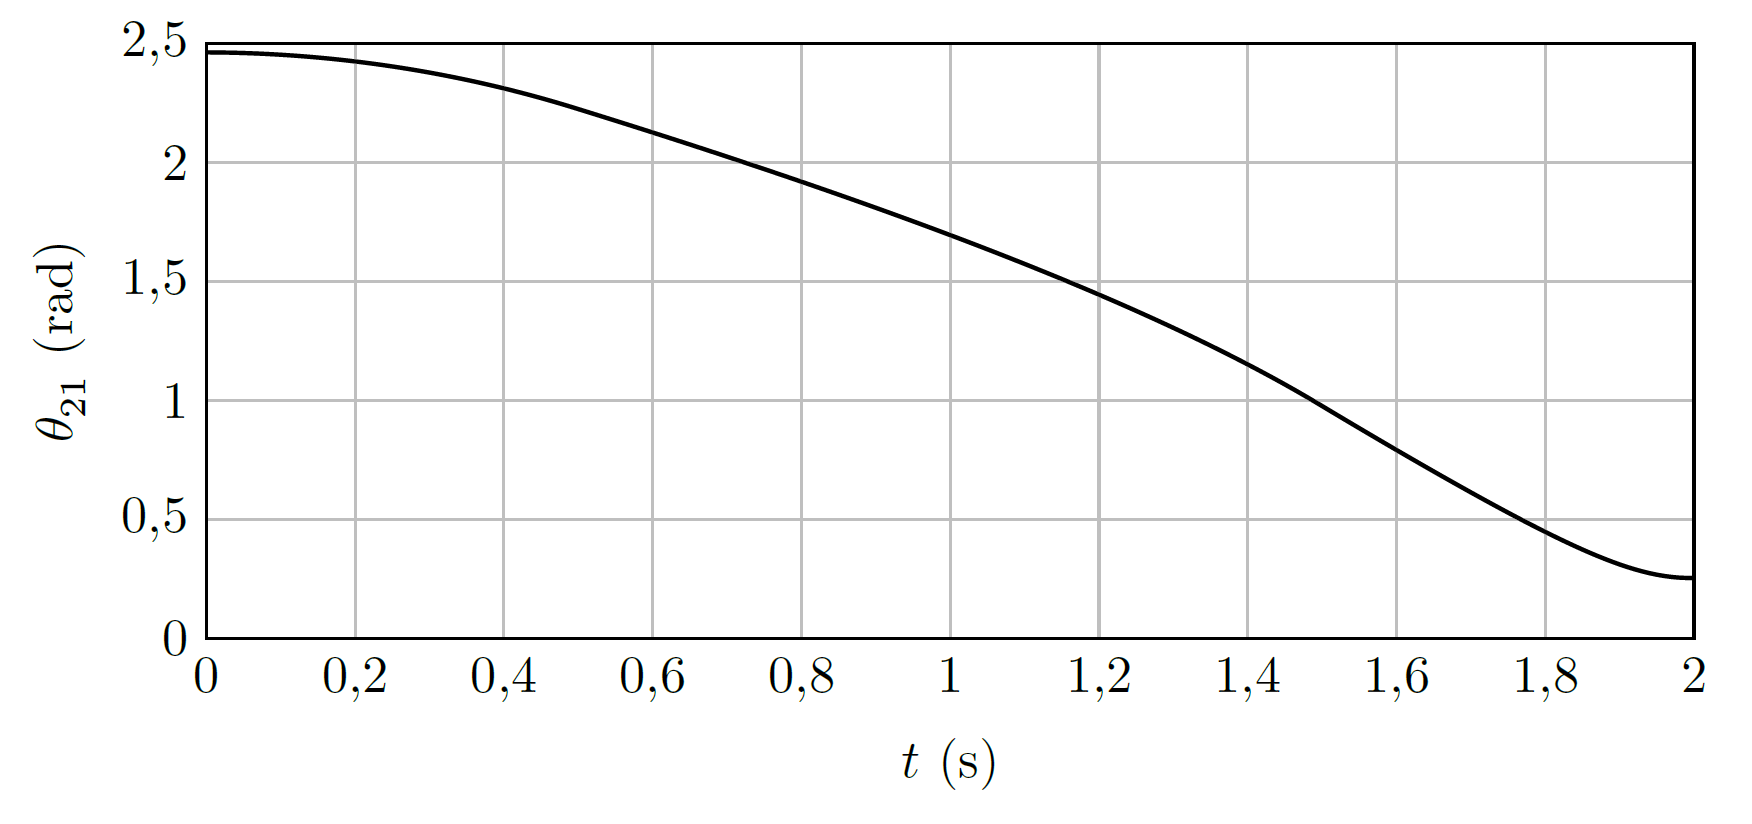
\includegraphics[width=0.8\linewidth]{img/fig06}
 \caption{Évolution de la consigne moteur}
 \label{img06}
\end{figure}

\begin{figure}[!h]
 \centering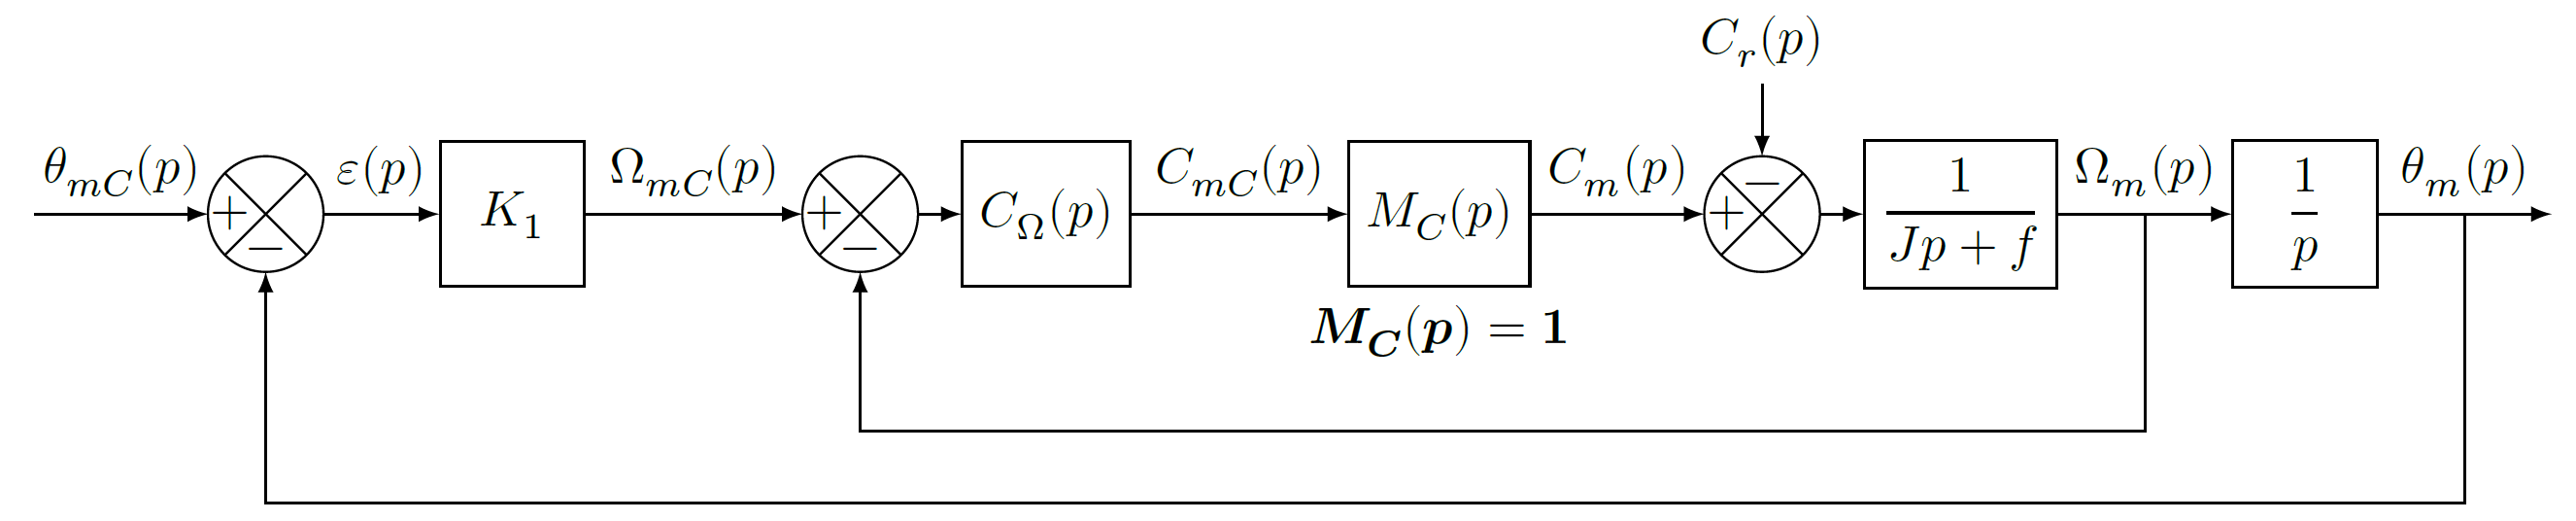
\includegraphics[width=1\linewidth]{img/fig07}
 \caption{Premier modèle}
 \label{img07}
\end{figure}

Selon le cahier des charges, pour assurer une bonne synchronisation des axes, l'exigence de précision statique
suite à une entrée de type échelon, de type rampe ou de type accélération doit être inférieure à 1\%.
Le premier modèle défini figure \ref{img07} est adopté pour chaque axe.

Notations:\\
\begin{tabular}{|c|l|}
\hline
$\theta_{mC}(p)$ &  consigne de position de l'axe moteur (variable temporelle : $\theta_{mC}(t)$ en $rad$), \\
\hline
$\theta_{m}(p)$ & position de l'axe moteur (variable temporelle : $\theta_{m}(t)$ en $rad$), \\
\hline
$C_{mC}(p)$ & consigne de couple moteur (variable temporelle : $C_{mC}(t)$ en $N.m$), \\
\hline
$C_{m}(p)$ & couple moteur (variable temporelle : $C_{m}(t)$ en $N.m$), \\
\hline
$C_{r}(p)$ & couple résistant perturbateur (variable temporelle : $C_{r}(t)$ en $N.m$), \\
\hline
$K_{1}$ & gain proportionnel du correcteur de l'asservissement de position (en $s^{-1}$), \\
\hline
$\Omega_{mC}(p)$ & consigne de vitesse de l'axe moteur (variable temporelle : $\Omega_{mC}(t)$ en $rad.s^{-1}$), \\
\hline
$\Omega_{m}(p)$ & vitesse de l'axe moteur (variable temporelle : $\Omega_{m}(t)$ en $rad.s^{-1}$), \\
\hline
$C_{\Omega}(p)$ & correcteur de l'asservissement de vitesse, \\
\hline
\multirow{2}{*}{$M_{C}(p)$} & modélise la boucle d'asservissement en couple de la machine électrique, \\
& considérée parfaite au vu de sa dynamique par rapport aux autres boucles : $M_{C}(p)=1$, \\
\hline
$J$ & moment d'inertie de l'ensemble en mouvement, rapporté au niveau de l'axe moteur, \\
\hline
$f$ & coefficient de frottements visqueux équivalent pour l'ensemble en mouvement. \\
\hline
\end{tabular}

~\

Le correcteur de l'asservissement de vitesse est de la forme $C_\Omega(p)=K_2.\frac{J.p+f}{J.p}$.

~\

Le premier modèle de la figure \ref{img07} permet de constater que :
\begin{itemize}
 \item l'écart est défini par la variable $\epsilon(t)=\theta_{mC}(t)-\theta_m(t)$,
 \item l'erreur entre l'entrée et la sortie est définie par la variable $\mu(t)=\theta_{mC}(t)-\theta_m(t)$.
\end{itemize}

\newpage

Étant donné que le modèle utilisé est à retour unitaire, l'écart $\epsilon(t)$ est égal à l'erreur $\mu(t)$.
La précision statique du système est définie par les paramètres suivants :
\begin{itemize}
 \item $\epsilon_p=\lim\limits_{t \rightarrow +\infty}\epsilon(t)$ suite à une entrée de type échelon unitaire $\theta_{mc}(t)=u(t)$, $\theta_{mc}(p)=\frac{1}{p}$, appelée erreur de position,
 \item $\epsilon_v=\lim\limits_{t \rightarrow +\infty}\epsilon(t)$ suite à une entrée de type rampe unitaire $\theta_{mc}(t)=t.u(t)$, $\theta_{mc}(p)=\frac{1}{p^2}$, appelée erreur de trainage,
 \item $\epsilon_a=\lim\limits_{t \rightarrow +\infty}\epsilon(t)$ suite à une entrée de type accélération $\theta_{mc}(t)=\frac{t^2}{2}.u(t)$, $\theta_{mc}(p)=\frac{1}{p^3}$, appelée erreur de accélération.
\end{itemize}

\paragraph{Hypothèse}

Le couple résistant évolue lentement au regard de la dynamique de l'asservissement, ce qui permet de considérer pour la suite de l'étude $C_r(tp)=0$.

\question{Déterminer la grandeur physique de la consigne et la grandeur physique asservie à partir du modèle multiphysique présenté figure \ref{img03} et préciser leurs unités de base dans le système international d'unités (SI).}

\question{Exprimer $H_\Omega=\frac{\Omega_m(p)}{\Omega_{mc}(p)}$ en fonction de $J$, $K_2$ et $p$.}

\question{Exprimer $\epsilon(p)$ en fonction de $\theta_{mC}(p)$, $H_\Omega(p)$, $K_1$ et $p$.}

\question{Déterminer l'erreur de position $\epsilon_p$ puis l'erreur de trainage $\epsilon_v$. Conclure sur la valeur de $K_1$ pour satisfaire à l'exigence d'erreur en trainage.}

\question{Déterminer l'erreur en accélération et conclure quant au respect du cahier des charges.}

~\

Pour satisfaire l'exigence d'une erreur en accélération inférieure à 1\%, le second modèle avec anticipation de la vitesse (figure \ref{img08}) est adopté avec $H_\Omega(p)=\frac{1}{1+T.p}$ et $T = 33 ms$.

\begin{figure}[!h]
 \centering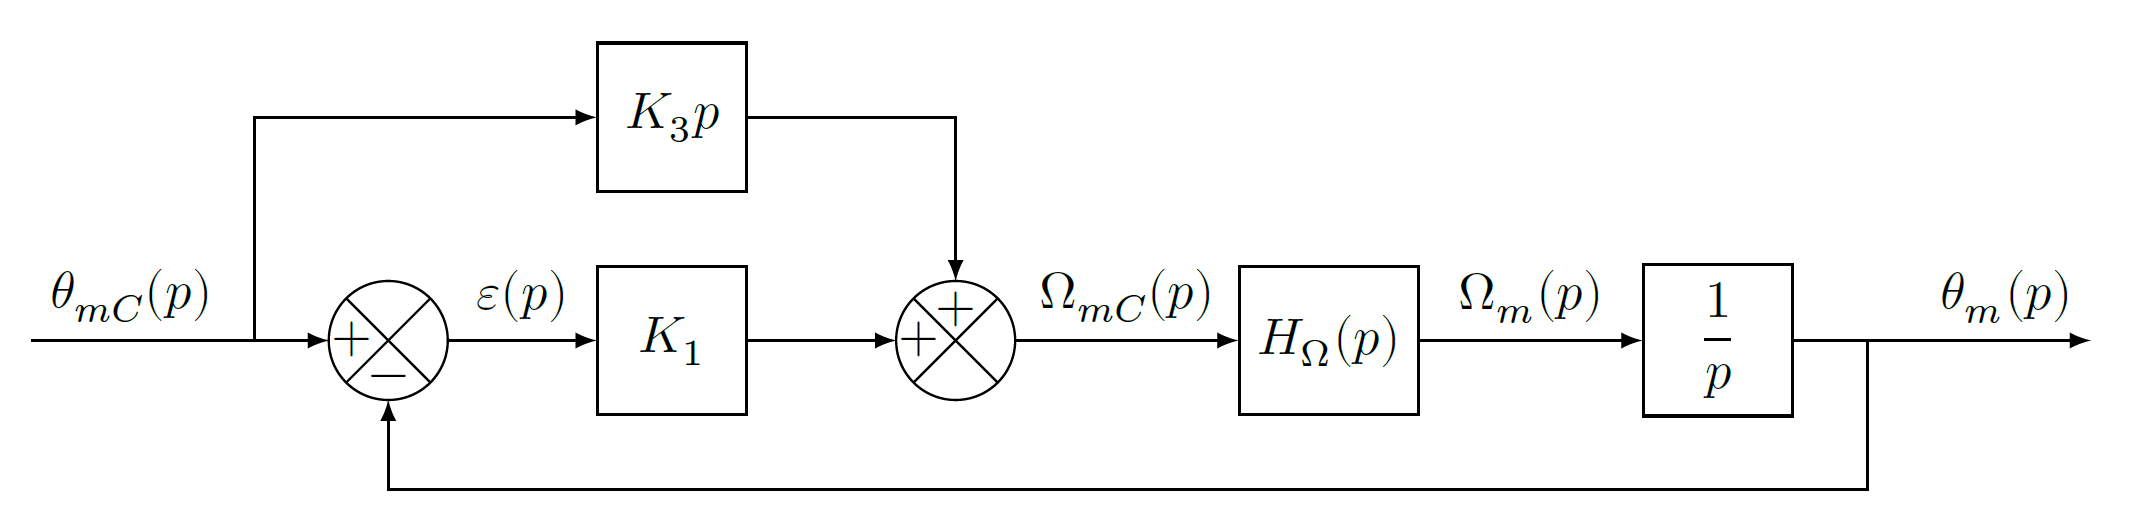
\includegraphics[width=0.9\linewidth]{img/fig08}
 \caption{Second modèle}
 \label{img08}
\end{figure}

\question{Exprimer $\epsilon(p)$ en fonction de $\theta_{mC}(p)$, $T$, $K_1$, $K_3$ et $p$.}

Le second modèle avec anticipation de la figure \ref{img08} n'a pas d'incidence sur la valeur de l'erreur de position.

\question{Exprimer l'erreur de trainage et déterminer la valeur de $K_3$ permettant d'annuler cette erreur.}

\question{Exprimer et déterminer l'erreur d'accélération en prenant les valeurs de $K_3$ et de $K_1$ déterminées précédemment. Conclure quant au respect du cahier des charges.}

\question{Déterminer la fonction de transfert $H(p)=\frac{\theta_m(p)}{\theta_{mC}(p)}$ à partie de la figure 8. Montrer qu'elle peut être mise sous la forme:

\begin{eqnarray}
H(p)=H_1(p)+H_2(p)=\frac{1}{1+\frac{p}{K_1}+\frac{T.p^2}{K_1}}+\frac{\frac{K_3.p}{K_1}}{1+\frac{p}{K_1}+\frac{T.p^2}{K_1}}
\end{eqnarray}}

\question{Déterminer les valeurs de $\omega_0$ et $\xi$.}

On donne, sur la figure \ref{img09}, le diagramme de Bode de la fonction de transfert $H_1(p)=\frac{1}{1+\frac{p}{K_1}+\frac{J.p^2}{K_1.K_2}}$.

\begin{figure}[!h]
 \centering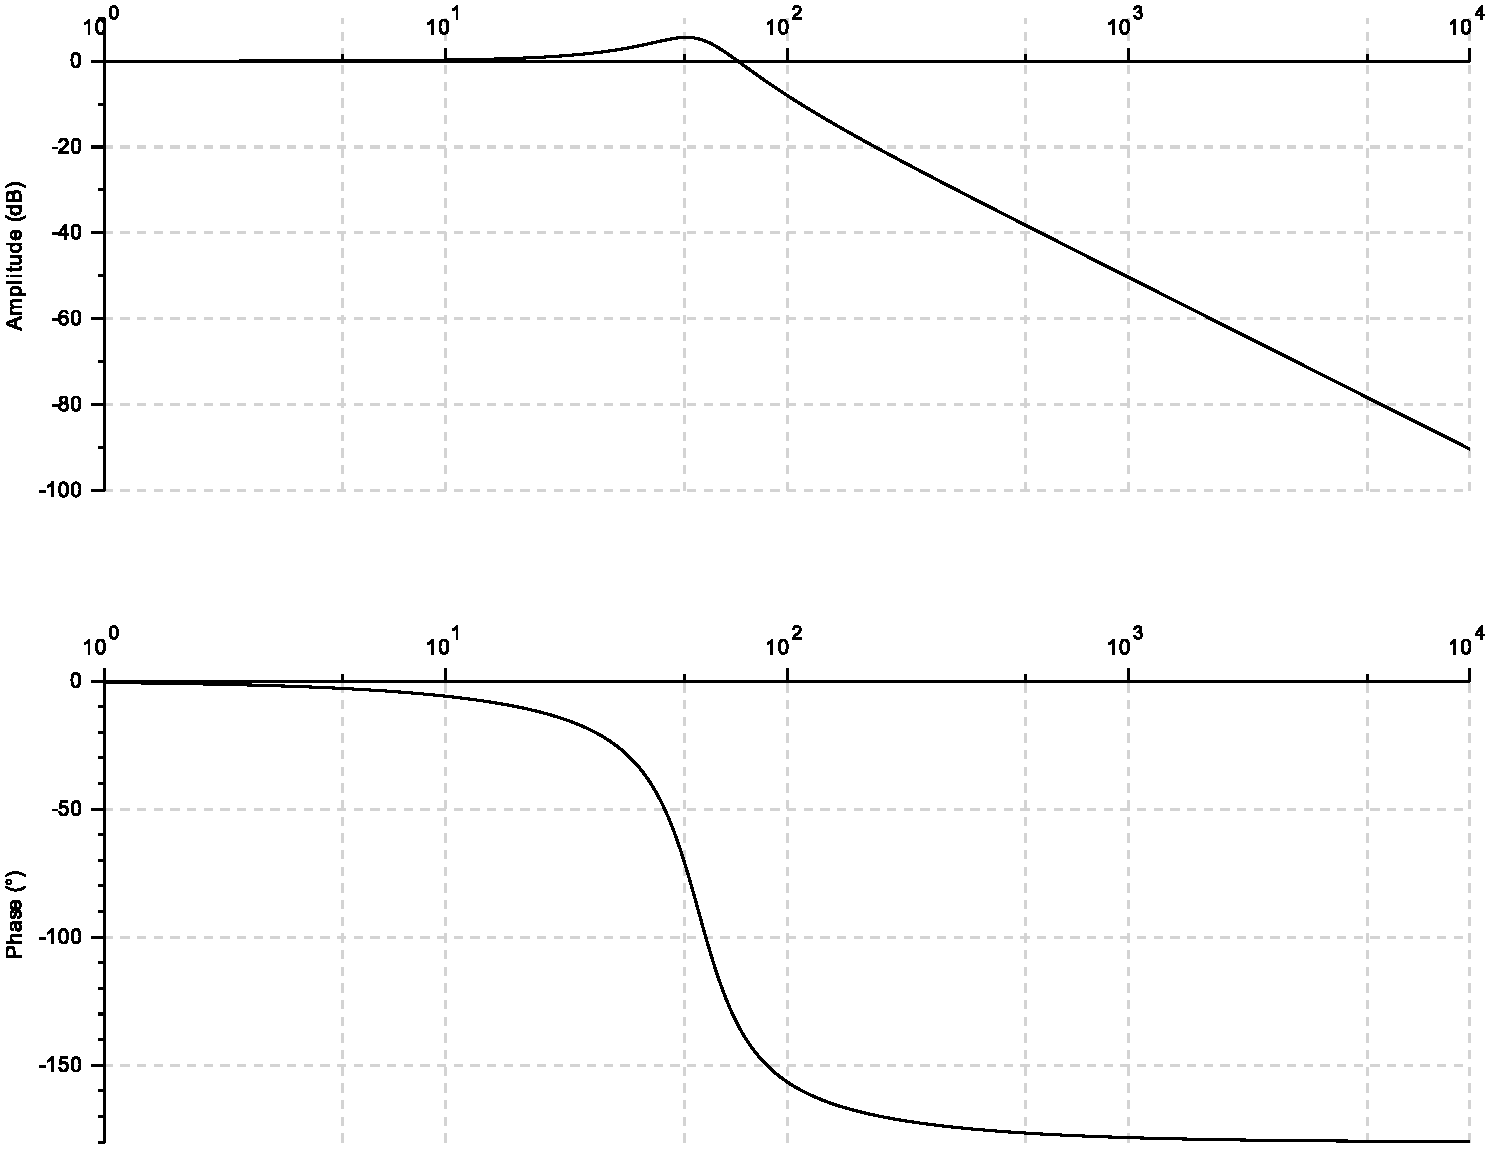
\includegraphics[width=0.8\linewidth]{img/bode1} \\ ~\ \\
 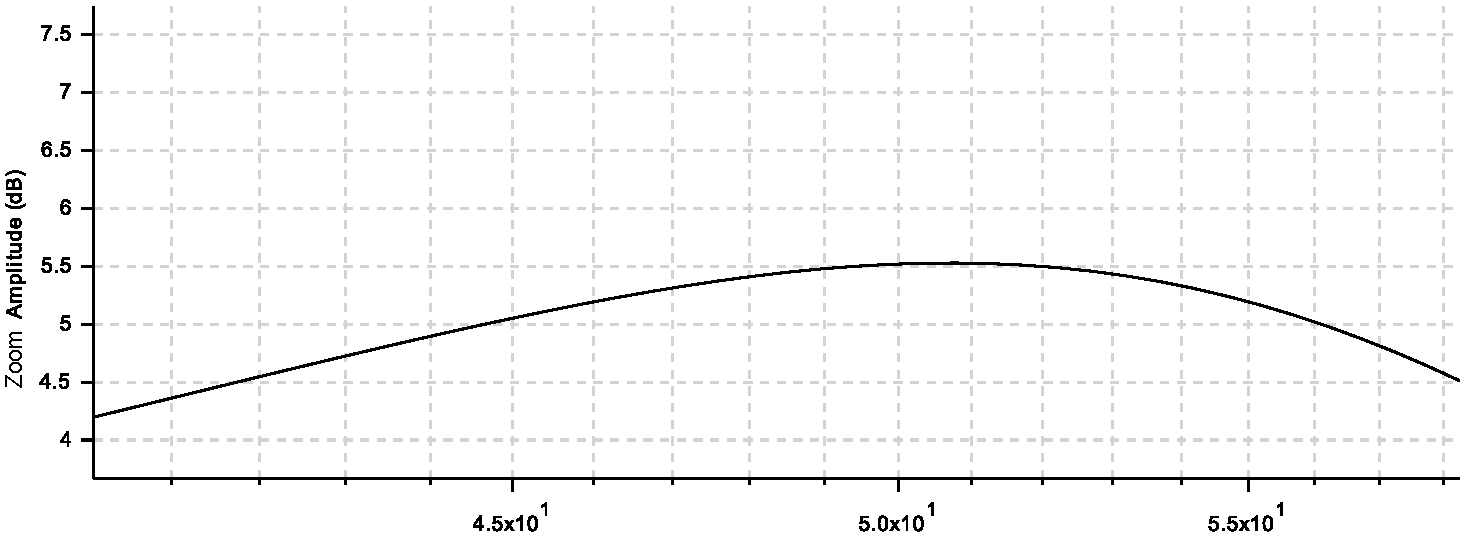
\includegraphics[width=0.8\linewidth]{img/bode1_2}
 \caption{Diagramme de Bode de $H_1(p)$}
 \label{img09}
\end{figure}

\question{Retrouver à partir du diagramme de Bode les valeurs de $\omega_0$ et $\xi$. Les comparer à celles trouvées précédemment.}

\question{Tracer, sur le document réponse, le diagramme de Bode de la fonction de transfert $H_2(p)$. Il est conseillé de s'appuyer sur celui de $H_1(p)$. Justifier les constructions.}

~\

On donne sur la figure \ref{img10} deux diagrammes de Bode.

\begin{figure}[!h]
 \centering	Tracé a \\
 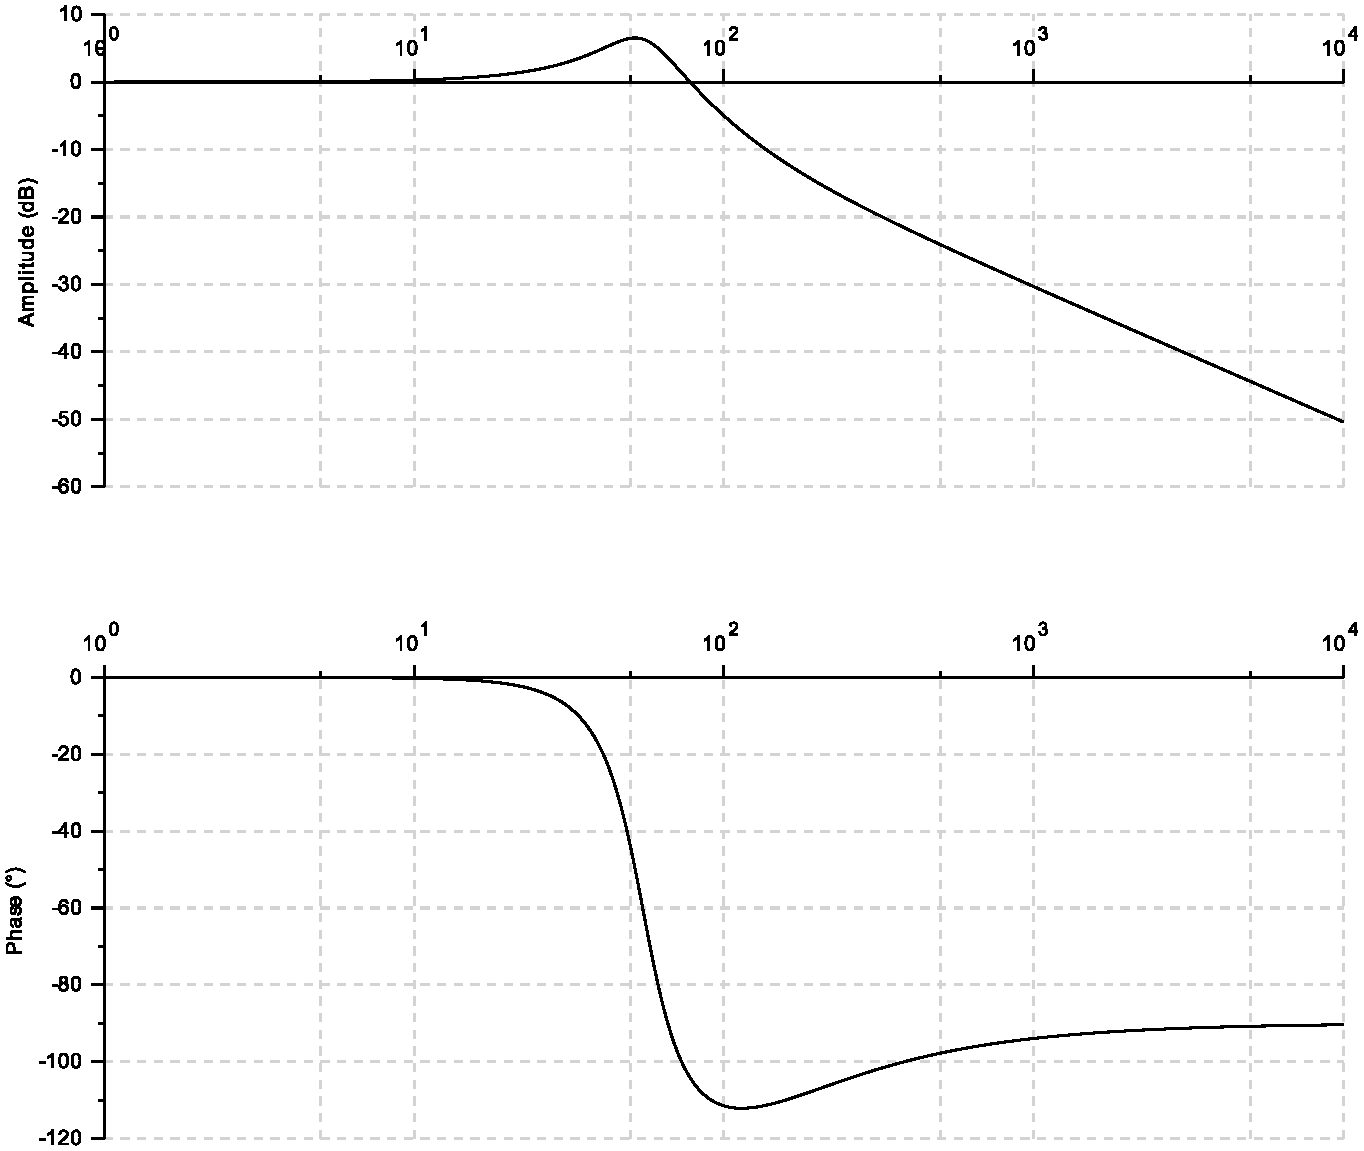
\includegraphics[width=0.7\linewidth]{img/bode3_1} \\ ~\ \\
 Tracé b \\
 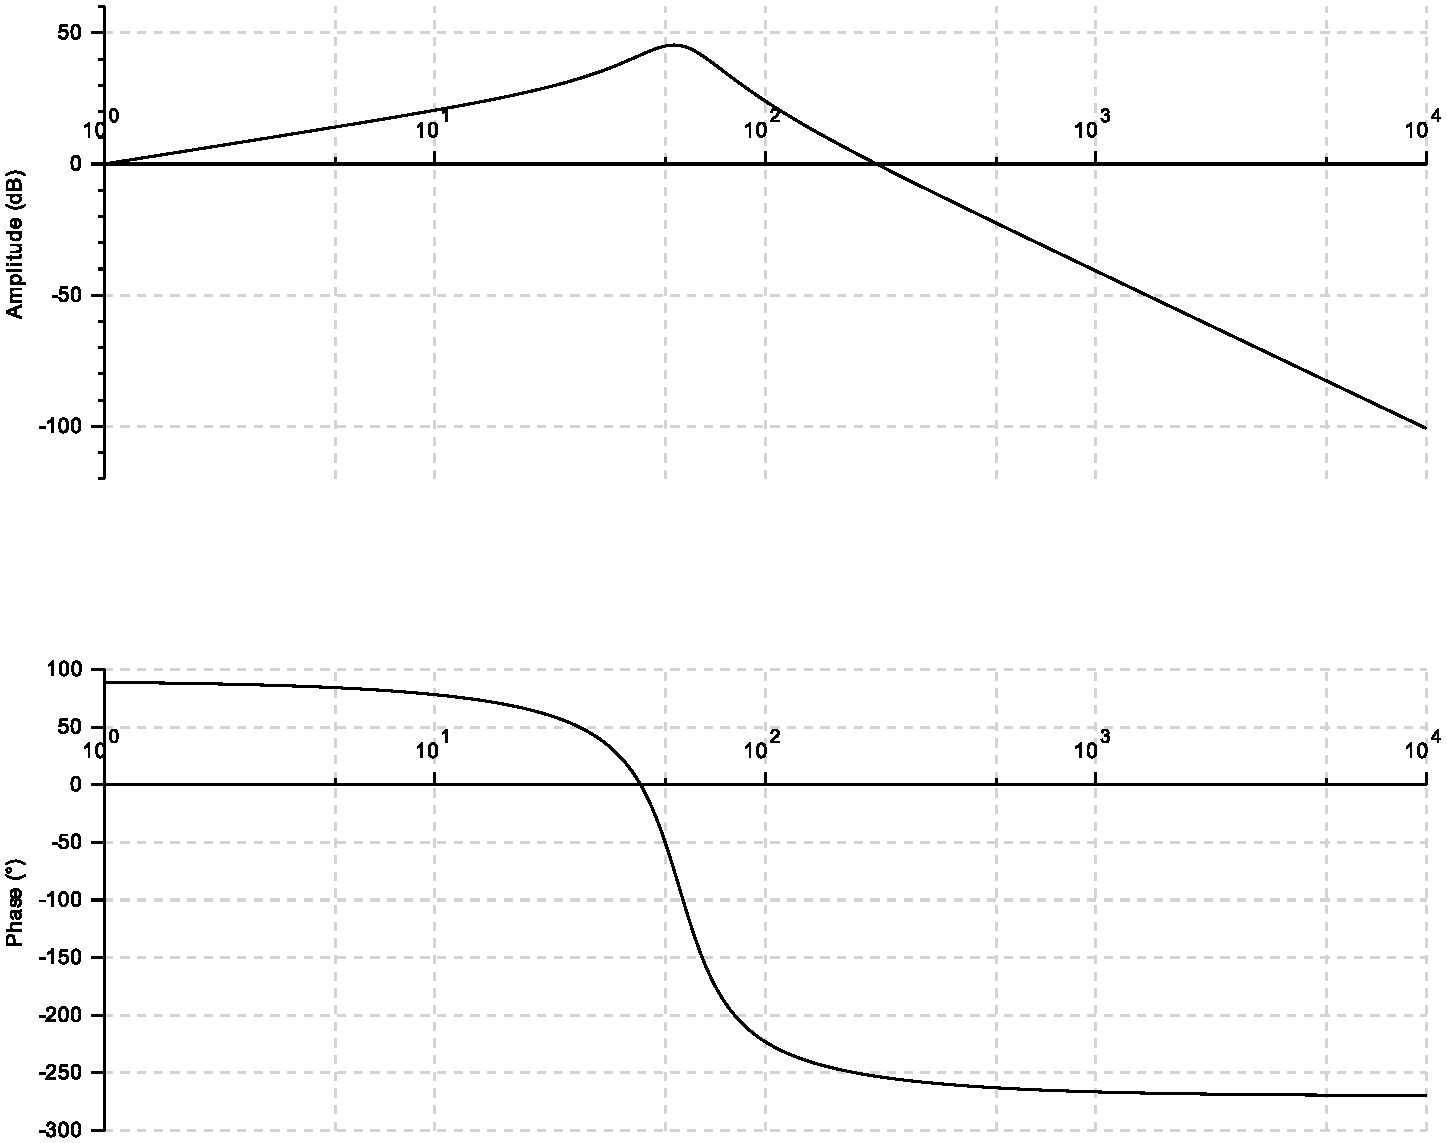
\includegraphics[width=0.7\linewidth]{img/bode3_2}
 \caption{Diagrammes de Bode pour $H(p)$}
 \label{img10}
\end{figure}

\question{Quel tracé correspond à celui de la fonction de transfert $H(p)$. Justifier.}

\section{Exercices supplémentaires}

\begin{figure}[!h]
 \centering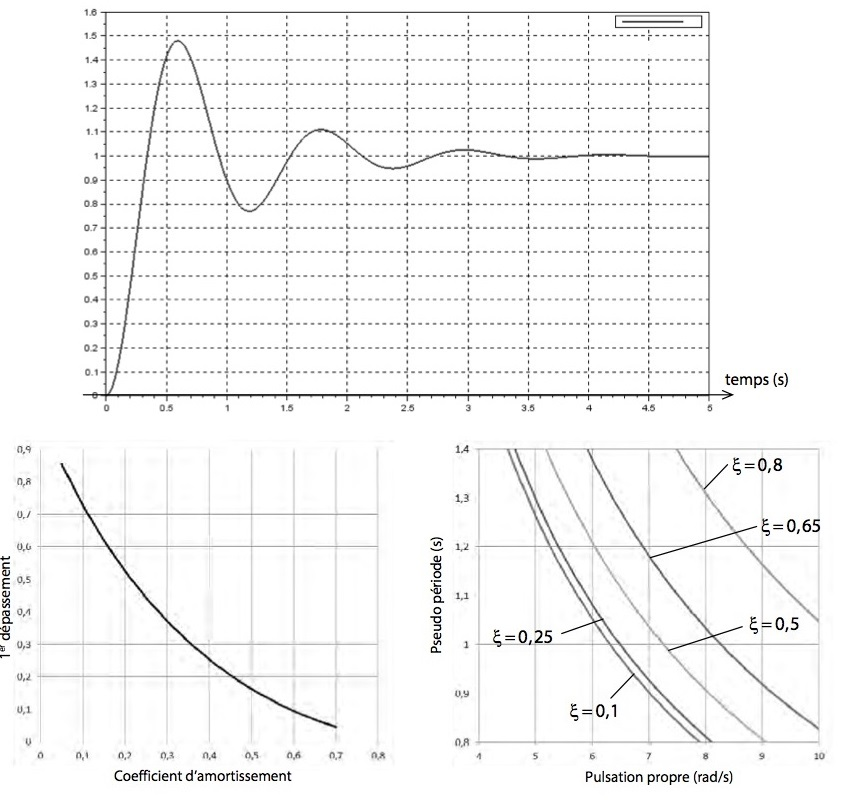
\includegraphics[width=0.9\linewidth]{img/fig09}
 \caption{Identification d'une fonction}
 \label{img11}
\end{figure}

\question{Identifier la fonction de transfert à partir de la réponse indicielle de la figure \ref{img11}. Déterminer à partir des abaques les valeurs numériques de $\xi$ et $\omega_0$. On indiquera toutes les constructions nécessaires sur les courbes.}

\newpage

\section{Conception d'un assemblage par vis}

\begin{figure}[!h]
 \centering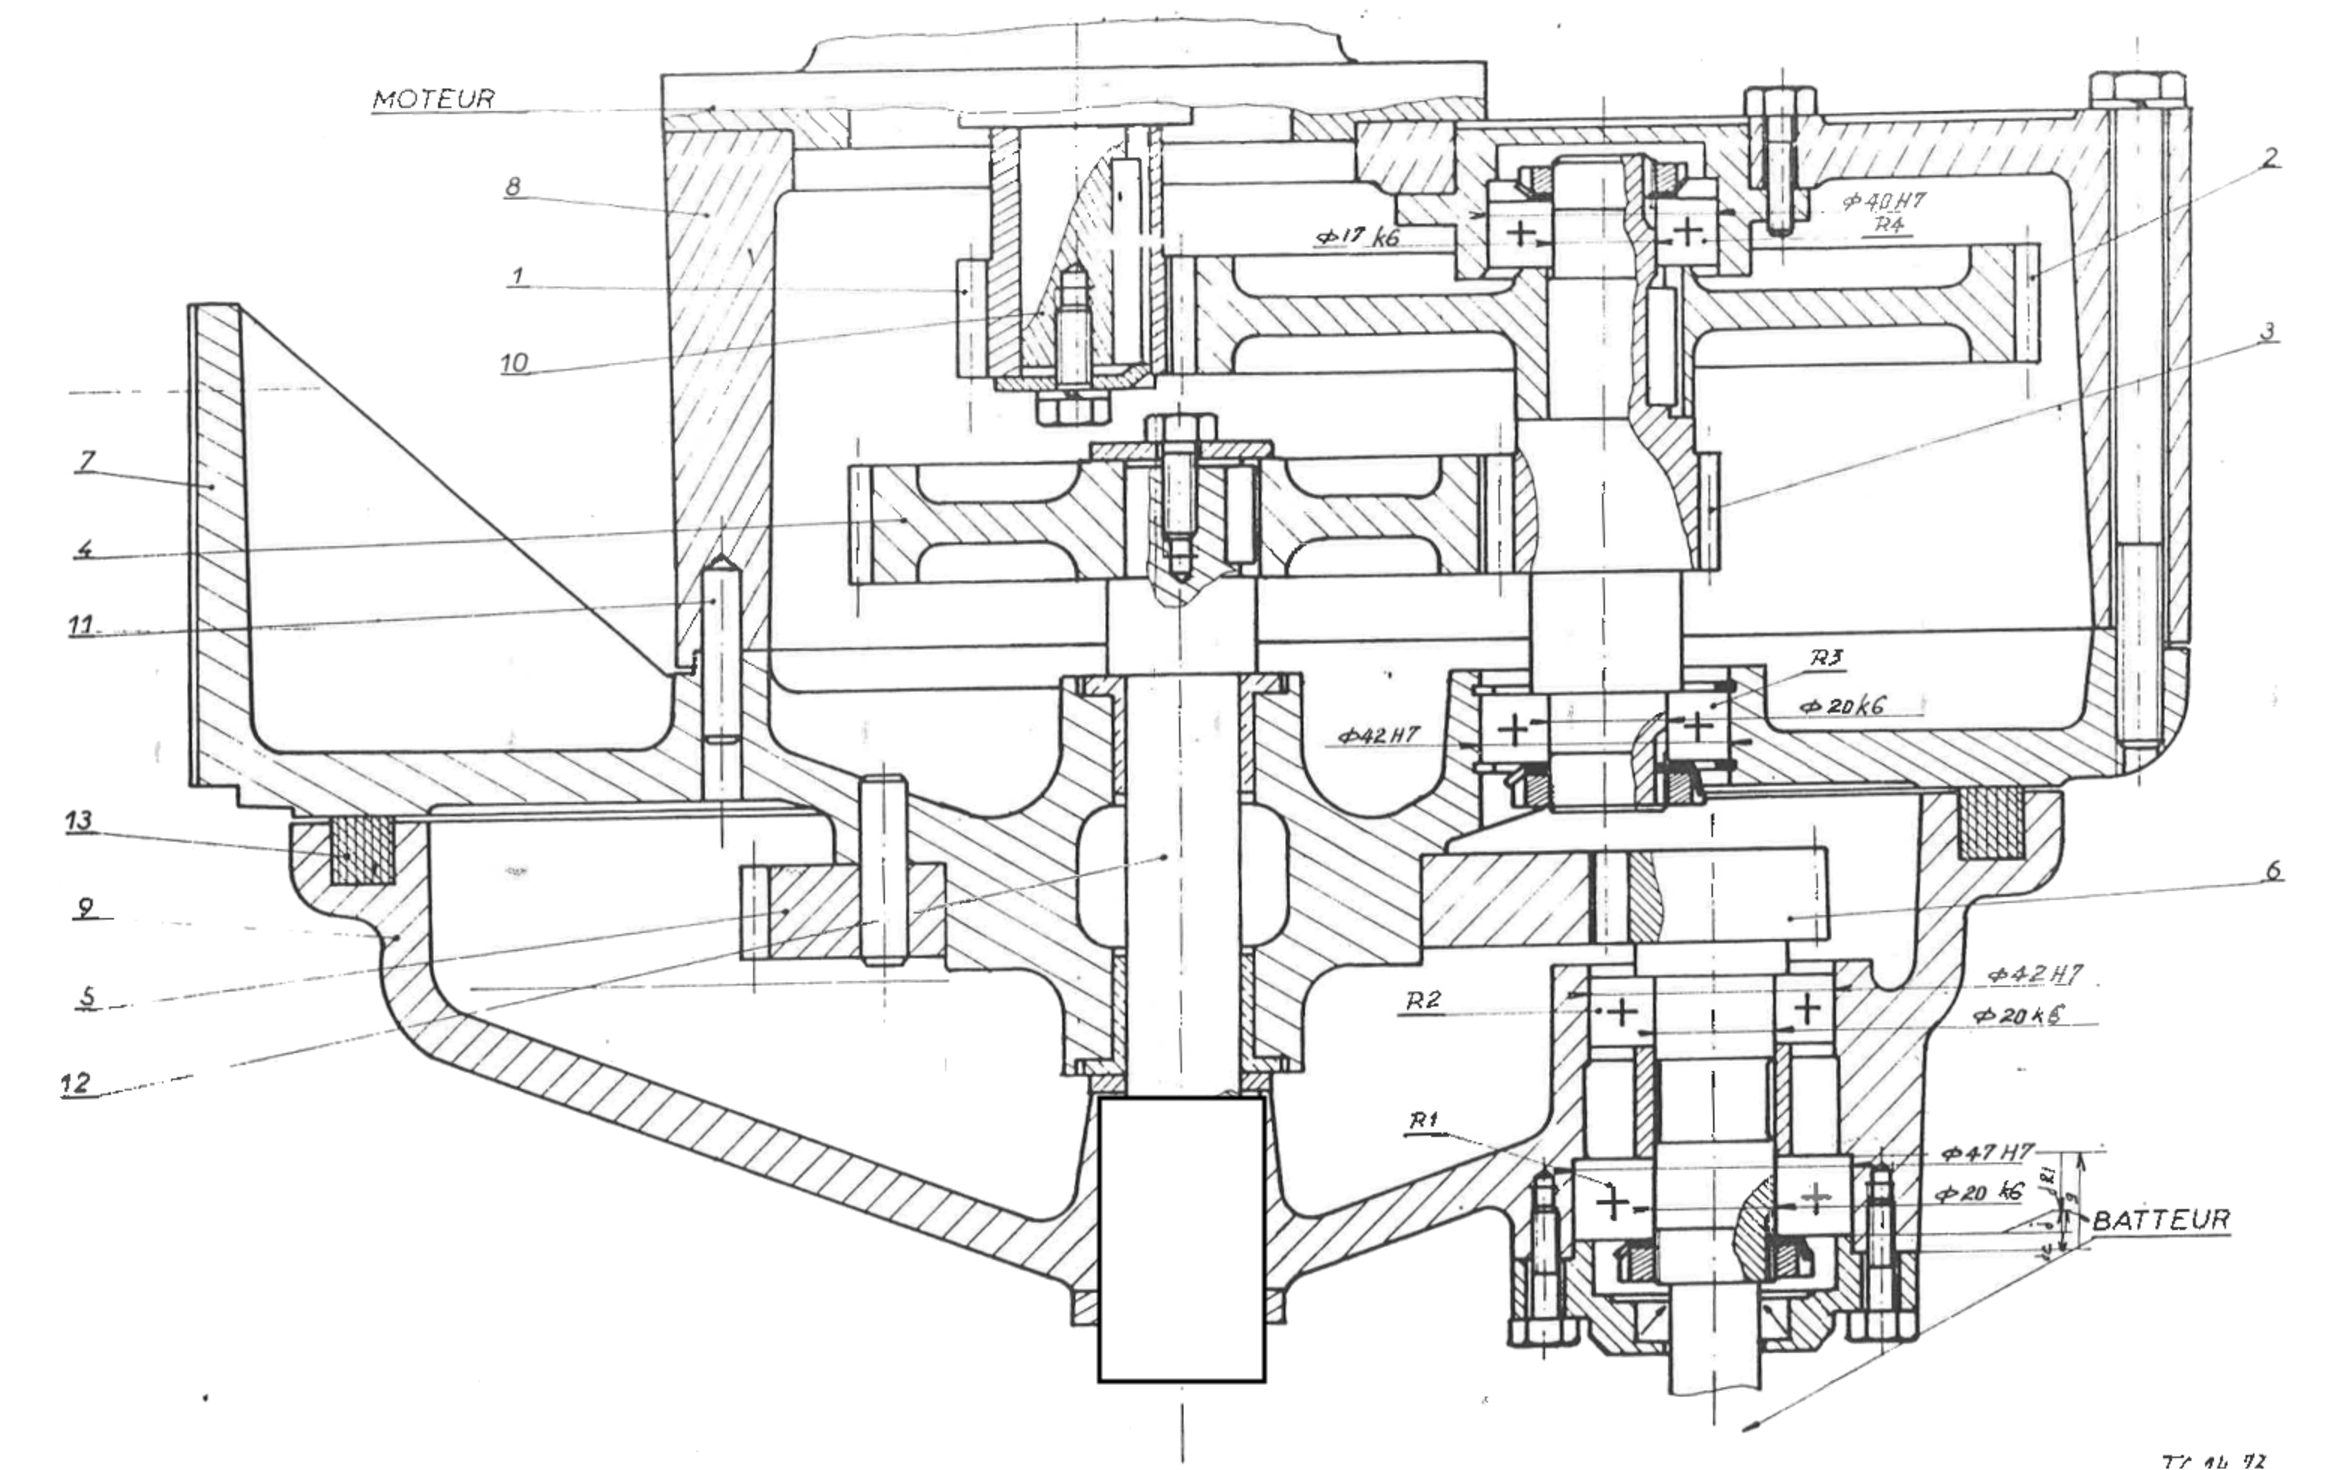
\includegraphics[width=0.9\linewidth]{img/Malaxeur_vierge}
 \caption{Conception d'un assemblage par vis}
 \label{img12}
\end{figure}

Au niveau de la zone à compléter, l'arbre 12 est cylindrique. Il est inséré dans un trou qui traverse la pièce 9. Une clavette empêche la rotation relative des deux pièces. Une vis traverse la pièce 9 et vient dans un taraudage percé dans la pièce 12. La solution demandée peut s'inspirer d'une autre zone du dessin.

\question{Compléter \textbf{le dessin du document réponse} en dessinant la solution d'assemblage vis+clavette dans le cadre prévu à cet effet.}

\cleardoublepage

\pagestyle{documentreponse}

\section{Documents réponse}

\reponse{14}

\reponse{12}

\reponse{10}

\newpage

\reponse{9}

\reponse{15}

\reponse{9}

\newpage

\reponse{9}

\reponse{8}

\reponse{11}

\reponse{11}

\newpage

\reponse{14}

\reponse{14}

\reponse{14}

\newpage

\reponse{13}

\reponse{13}

\reponse{11}

\newpage

\reponse{5}

\begin{center}
	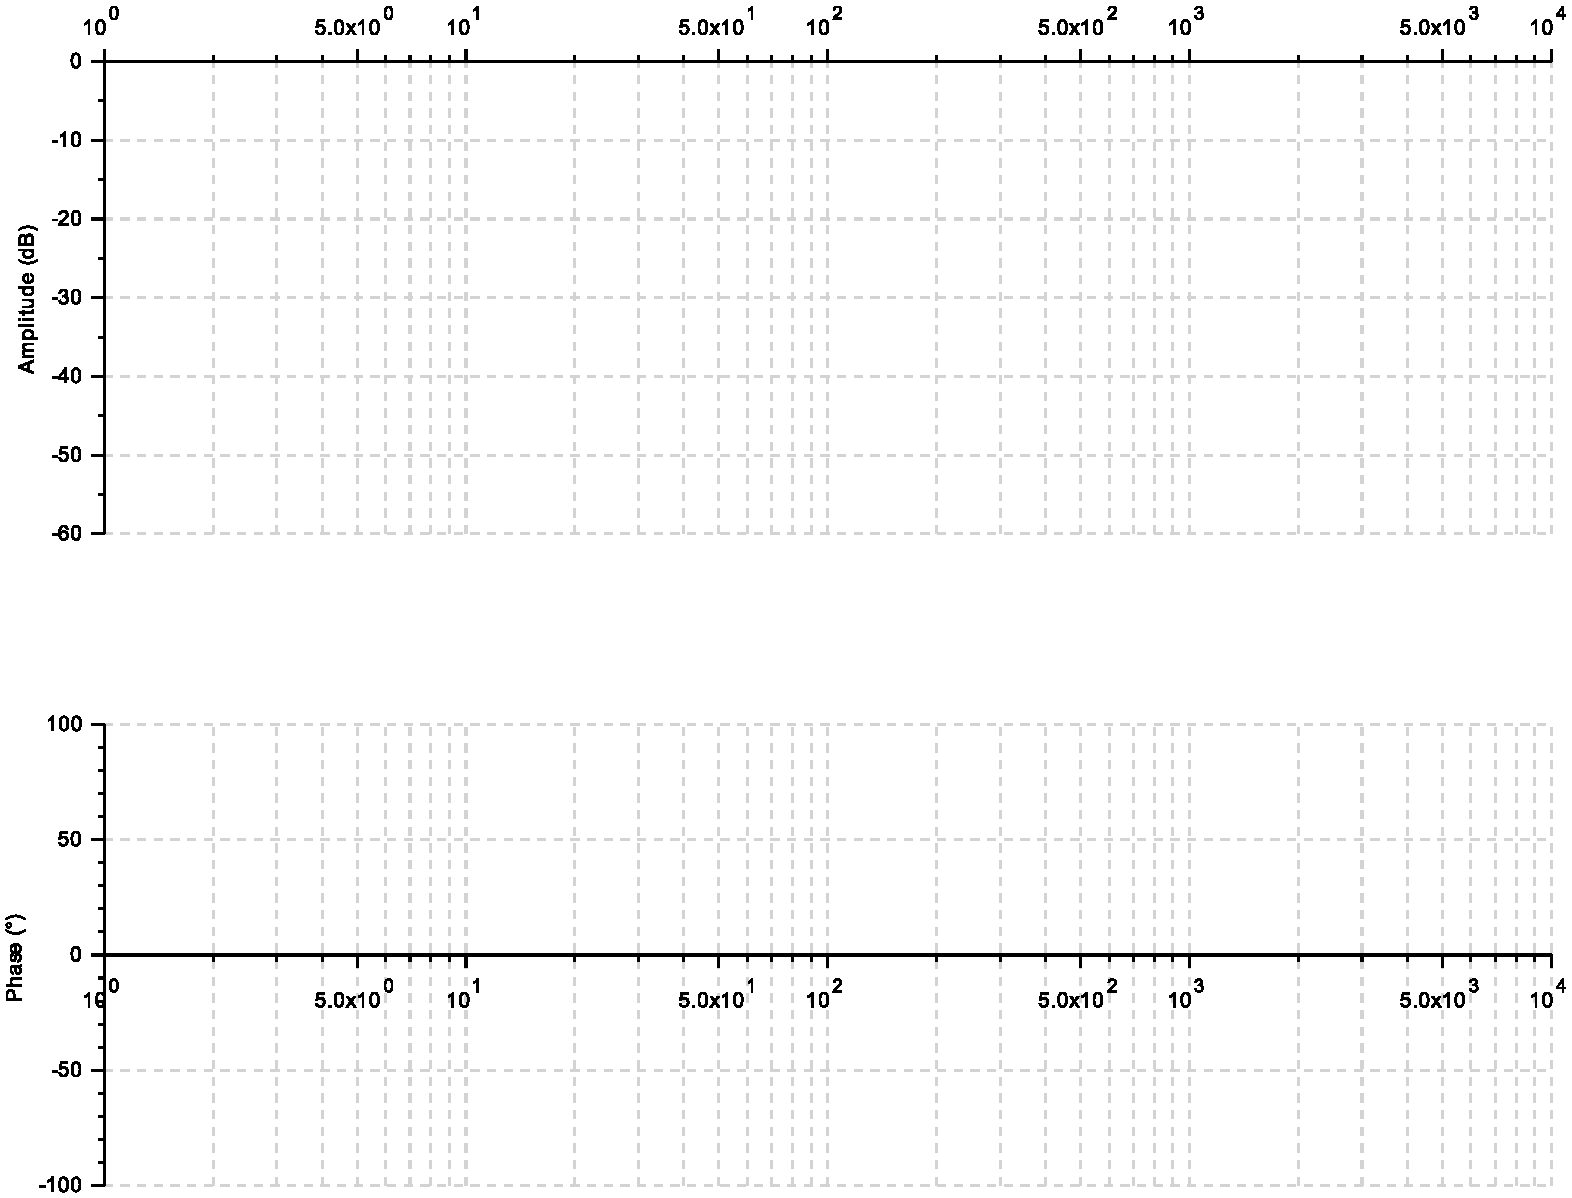
\includegraphics[width=0.9\linewidth]{img/bode2}
\end{center}

\reponse{9}

\newpage

\reponse{9}

\reponse{5}

\begin{center}
	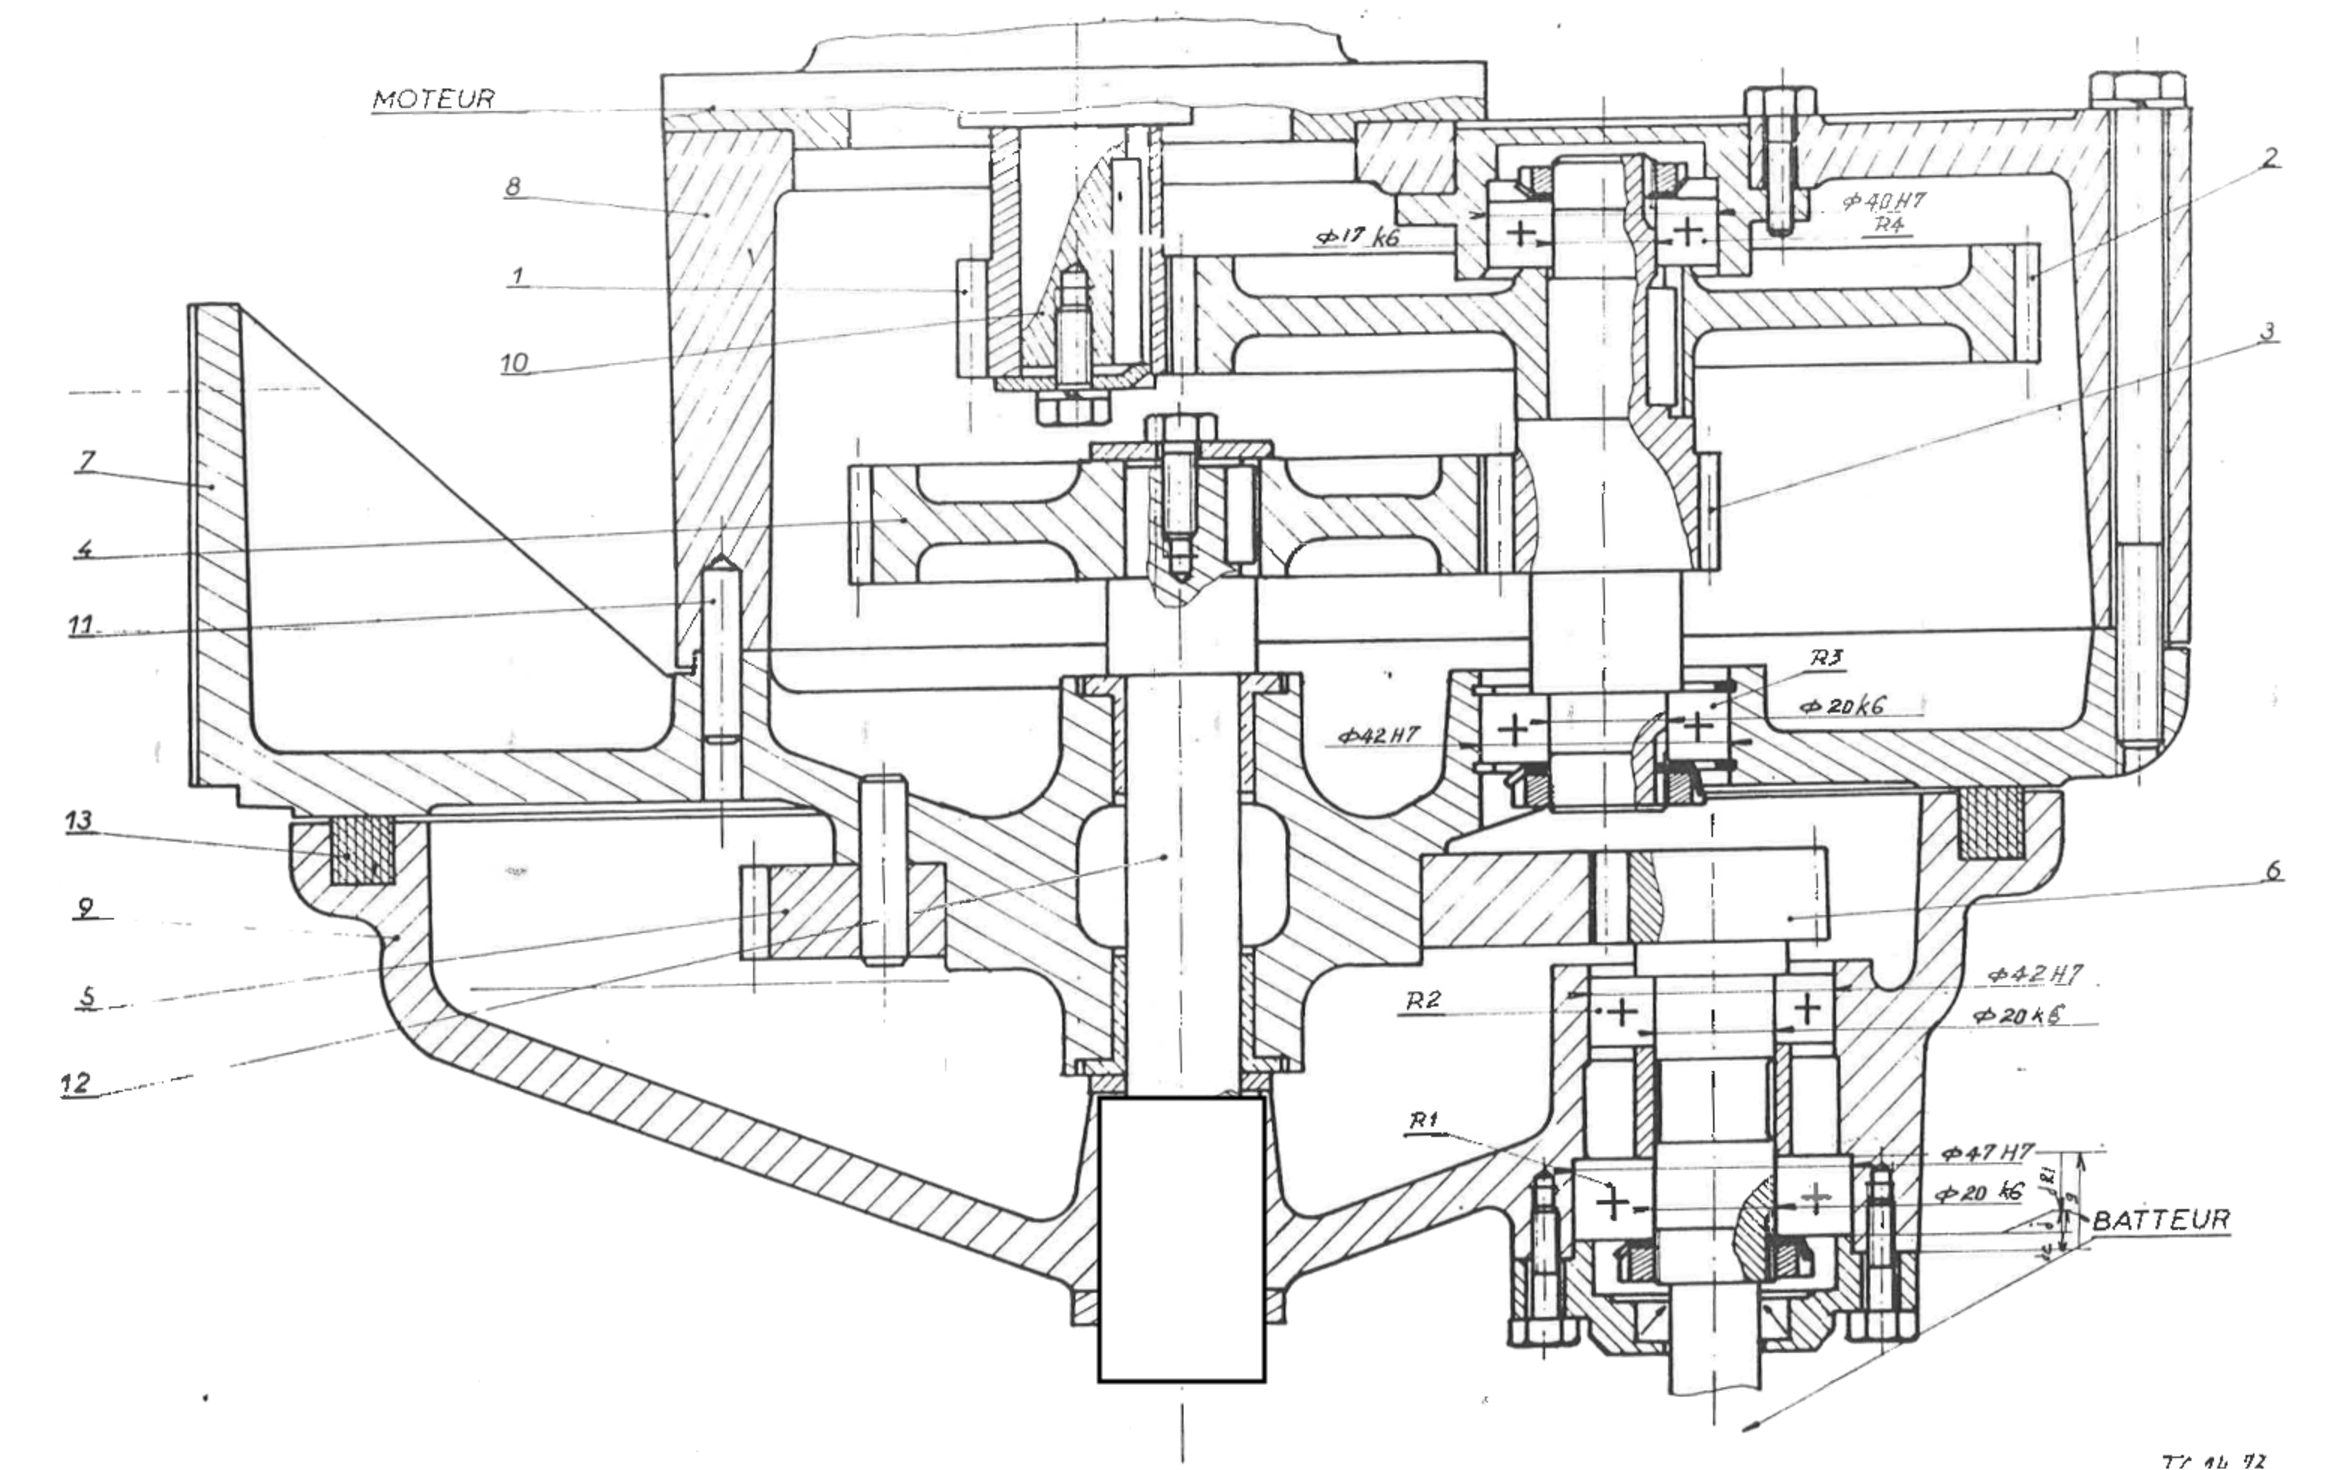
\includegraphics[width=0.9\linewidth]{img/Malaxeur_vierge}
\end{center}

\ifdef{\public}{\end{document}}{}

\newpage
\cleardoublepage

\pagestyle{correction}

\setcounter{equation}{0}

\section{Correction}

\cor

Fermeture géométrique:
$\overrightarrow{O_0A}+\overrightarrow{AO_1}+\overrightarrow{O_1O_2}+\overrightarrow{O_2O_0}=\overrightarrow{0}$

$l_4.\overrightarrow{y_0}+L.\overrightarrow{y_1}+l_1.\overrightarrow{y_2}-h(t).\overrightarrow{z_0}=\overrightarrow{0}$

Après les projections, ont trouve:
\begin{eqnarray}
l_4=-L.cos\theta_{10}-l_1.cos(\theta_{10}+\theta_{21}) \label{coreq1}\\
h(t)=L.sin\theta_{10}+l_1.sin(\theta_{10}+\theta_{21}) \label{coreq2}
\end{eqnarray}

\cor

En faisant (\ref{coreq1})$^2$+( \ref{coreq2})$^2$:

$l_4^2+h(t)^2=L^2+2.L.l_1.\left[cos(\theta_{10}+\theta_{21}).cos\theta_{10}+sin(\theta_{10}+\theta_{21}).sin\theta_{10}\right]+l_1^2$

Et ainsi, $\theta_{21}=arccos\left(\frac{l_4^2+h(t)^2-L^2-l_1^2}{2.L.l_1}\right)$

\cor

Comme pour la question précédente, on obtient:

$2.L.l_4.cos\theta_{10}-2.L.h(t).sin\theta_{10}=l_1^2-h(t)^2-L^2-l_4^2$

En posant $cos(\varphi)=\frac{l_4}{\sqrt{l_4^2+h(t)^2}}$ et $sin(\varphi)=\frac{-h(t)}{\sqrt{l_4^2+h(t)^2}}$, on en déduit:

$cos(\theta_{10}-\varphi)=\frac{l_1^2-h(t)^2-L^2-l_4^2}{2.L.\sqrt{l_4^2+h(t)^2}}$ et $\varphi=arctan\left(-\frac{h(t)}{l_4}\right)$

Finalement: $\theta_{10}=arccos\left(\frac{l_1^2-h(t)^2-L^2-l_4^2}{2.L.\sqrt{l_4^2+h(t)^2}}\right)+arctan\left(-\frac{h(t)}{l_4}\right)$

\cor

\begin{center}
 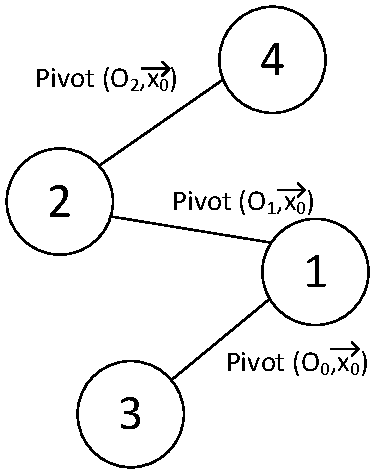
\includegraphics[width=0.4\linewidth]{img/graphe_liaisons}
\end{center}

\cor

$\left\{V_{1/3}\right\}=\left\{\begin{array}{cc}
\omega_{13x} & 0 \\
0 & 0 \\
0 & 0
\end{array}\right\}_{O_0,R_0(\overrightarrow{x_0},\overrightarrow{y_0},\overrightarrow{z_0})}$,
$\left\{V_{2/1}\right\}=\left\{\begin{array}{cc}
\omega_{21x} & 0 \\
0 & 0 \\
0 & 0
\end{array}\right\}_{O_1,R_0(\overrightarrow{x_0},\overrightarrow{y_0},\overrightarrow{z_0})}$
$\left\{V_{4/2}\right\}=\left\{\begin{array}{cc}
\omega_{42x} & 0 \\
0 & 0 \\
0 & 0
\end{array}\right\}_{O_2,R_0(\overrightarrow{x_0},\overrightarrow{y_0},\overrightarrow{z_0})}$

$\left\{T_{1\rightarrow 3}\right\}=\left\{\begin{array}{cc}
X_{13} & 0 \\
Y_{13} & M_{13} \\
Z_{13} & N_{13}
\end{array}\right\}_{O_0,R_0(\overrightarrow{x_0},\overrightarrow{y_0},\overrightarrow{z_0})}$
$\left\{T_{2\rightarrow 1}\right\}=\left\{\begin{array}{cc}
X_{21} & 0 \\
Y_{21} & M_{21} \\
Z_{21} & N_{21}
\end{array}\right\}_{O_1,R_0(\overrightarrow{x_0},\overrightarrow{y_0},\overrightarrow{z_0})}$
$\left\{T_{4\rightarrow 2}\right\}=\left\{\begin{array}{cc}
X_{42} & 0 \\
Y_{42} & M_{42} \\
Z_{42} & N_{42}
\end{array}\right\}_{O_2,R_0(\overrightarrow{x_0},\overrightarrow{y_0},\overrightarrow{z_0})}$

\cor

En regardant le modèle multiphysique, on voit que:
\begin{itemize}
 \item on mesure la coordonnée verticale de l'articulation de la hanche (en m),
 \item on donne en consigne la vitesse de déplacement vertical de la hanche (en m.s$^{-1}$).
\end{itemize}

\cor

En prenant $C_R(p)=0$,

$H_\Omega(p)=\frac{\Omega_m(p)}{\Omega_{mC}(p)}=\frac{C_\Omega(p).M_C(p).\frac{1}{J.p+f}}{1+C_\Omega(p).M_C(p).\frac{1}{J.p+f}}=\frac{\frac{K_2}{J.p}}{1+\frac{K_2}{J.p}}=\frac{1}{1+\frac{J}{K_2}.p}$

\cor

$\epsilon(p)=\frac{1}{1+K_1.H_\Omega(p).\frac{1}{p}}.\theta_{mc}(p)$

\cor

Erreur de position: $\epsilon_p=\lim\limits_{p\rightarrow 0}p.\epsilon(p)=\lim\limits_{p\rightarrow 0}=\frac{1}{1+K_1.H_\Omega(p).\frac{1}{p}}=0$

Erreur de trainage: $\epsilon_v=\lim\limits_{p\rightarrow 0}p.\epsilon(p)=\lim\limits_{p\rightarrow 0}=\frac{1}{1+K_1.H_\Omega(p).\frac{1}{p}}.\frac{1}{p}=\frac{1}{K_1}$

Pour $\epsilon_v<1\%$, il faut $K_1=100$.

\cor

Erreur d'accélération: $\epsilon_a=\lim\limits_{p\rightarrow 0}p.\epsilon(p)=\lim\limits_{p\rightarrow 0}=\frac{1}{1+K_1.H_\Omega(p).\frac{1}{p}}.\frac{1}{p^2}=+\infty$

Dans ce cas, le cahier des charges n'est pas respecté.

\cor

En utilisant le second modèle,

$\epsilon(p)=\theta_{mc}(p)-\theta_{m}(p)=\theta_{mc}(p)-\left(K_1.\epsilon(p)+K_3.p.\theta_{mc}(p)\right).H_\Omega(p).\frac{1}{p}$

$\epsilon(p)=\frac{1-K_3.H_\Omega(p)}{1+K_1.H_\Omega(p).\frac{1}{p}}.\theta_{mc}(p)=\frac{1-\frac{K_3}{1+T.p}}{1+\frac{K_1}{(1+(T.p).p}}\theta_{mc}(p)=\frac{1+T.p-K_3}{T.p^2+p+K_1}.p.\theta_{mc}(p)$

\cor

$\epsilon_v=\lim\limits_{p\rightarrow 0}p.\epsilon(p)=\lim\limits_{p\rightarrow 0}\frac{1+T.p-K_3}{T.p^2+p+K_1}=\frac{1-K_3}{K_1}$

Pour $\epsilon_v=0$, $K_3=1$.

\cor

$\epsilon(p)=\frac{T.p}{T.p^2+p+100}.p.\theta_{mc}(p)$

$\epsilon_a=\lim\limits_{p\rightarrow 0}p.\epsilon(p)=\lim\limits_{p\rightarrow 0}\frac{T}{T.p^2+p+100}=\frac{T}{100}=33.10^{-5}$

Ce résultat est compatible avec le cahier des charges.

\cor

D'après le schéma bloc:\\
$\theta_m(p)=\left(\theta_{mc}(p).K_3.p+\left(\theta_{mc}(p)-\theta_{m}(p)\right).K_1\right).H_\Omega(p).\frac{1}{p}$

$\theta_m(p)\left(1+K_1.H_\Omega(p).\frac{1}{p}\right)=\left(\theta_{mc}(p).K_3.p+\theta_{mc}(p).K_1\right).H_\Omega(p).\frac{1}{p}$

$\frac{\theta_m(p)}{\theta_{mc}(p)}=\frac{\left(K_3.p+K_1\right).H_\Omega(p).\frac{1}{p}}{1+K_1.H_\Omega(p).\frac{1}{p}}$

$\frac{\theta_m(p)}{\theta_{mc}(p)}=\frac{\left(K_3.p+K_1\right).\frac{1}{1+T.p}.\frac{1}{p}}{1+K_1.\frac{1}{1+T.p}.\frac{1}{p}}$

$\frac{\theta_m(p)}{\theta_{mc}(p)}=\frac{\frac{K_3.p+K_1}{K_1}}{1+\frac{p}{K_1}+\frac{T.p^2}{K_1}}$

$\frac{\theta_m(p)}{\theta_{mc}(p)}=\frac{1}{1+\frac{p}{K_1}+\frac{T.p^2}{K_1}}+\frac{\frac{K_3.p}{K_1}}{1+\frac{p}{K_1}+\frac{T.p^2}{K_1}}$

\cor

$\omega_0=\sqrt{\frac{K_1}{T}}=\sqrt{\frac{100}{33.10^{-3}}}=\sqrt{3.10^3}=\sqrt{3.10}.10\simeq 1,7.3.10 \simeq 51$

$\frac{2.\xi}{\omega_0}=\frac{1}{K_1}$, donc $\xi=\frac{\omega_0}{2.K_1}=\frac{51}{2.100}\simeq0,25$

\cor

$20.logQ=5,5$

$Q=10^{\frac{5,5}{20}}\simeq 10^{\frac{1}{4}}\simeq\sqrt{3}$

$Q=\frac{1}{2.\xi.\sqrt{1-\xi^2}}$

Donc, $3=\frac{1}{4.\xi^2.(1-\xi^2)}$, en prenant $\xi^2=x$, on a 

$x^2-x+\frac{1}{12}=0$

$\Delta=1-4.\frac{1}{12}=\frac{2}{3}$

$x_1=\frac{1+\sqrt{\frac{2}{3}}}{2}=\frac{1,8}{2}=0,9$

$x_2=\frac{1-\sqrt{\frac{2}{3}}}{2}=\frac{0,2}{2}=0,1$

Donc, $\xi=\sqrt{0,1}\simeq 0,3$

$\omega_r=\omega_0.\sqrt{1-2.\xi^2}$

$\omega_0=\frac{\omega_r}{\sqrt{1-2.\xi^2}}=\frac{50}{\sqrt{0,8}}=\frac{50}{0,9}=55,55$

On retrouve des valeurs proches de celles calculées précédemment.

\cor

La nouvelle fonction de transfert est $H_2(p)=\frac{\frac{K_3.p}{K_1}}{1+\frac{p}{K_1}+\frac{T.p^2}{K_1}}$.

Il s'agit de la première $H_1(p)$, multipliée par $\frac{K_3.p}{K_1}$.

La courbe de l'amplitude est décalée vers le bas de $20.log\frac{K_3}{K_1}=-20.2=-40$. Il faut ensuite ajouter la droite $20.log\omega$, soit une pente de $20dB/dec$ qui coupe l'axe des abscisses pour $\omega=1rad.s^{-1}$.

La courbe de la phase est décalée de 90° vers le haut.

\begin{center}
 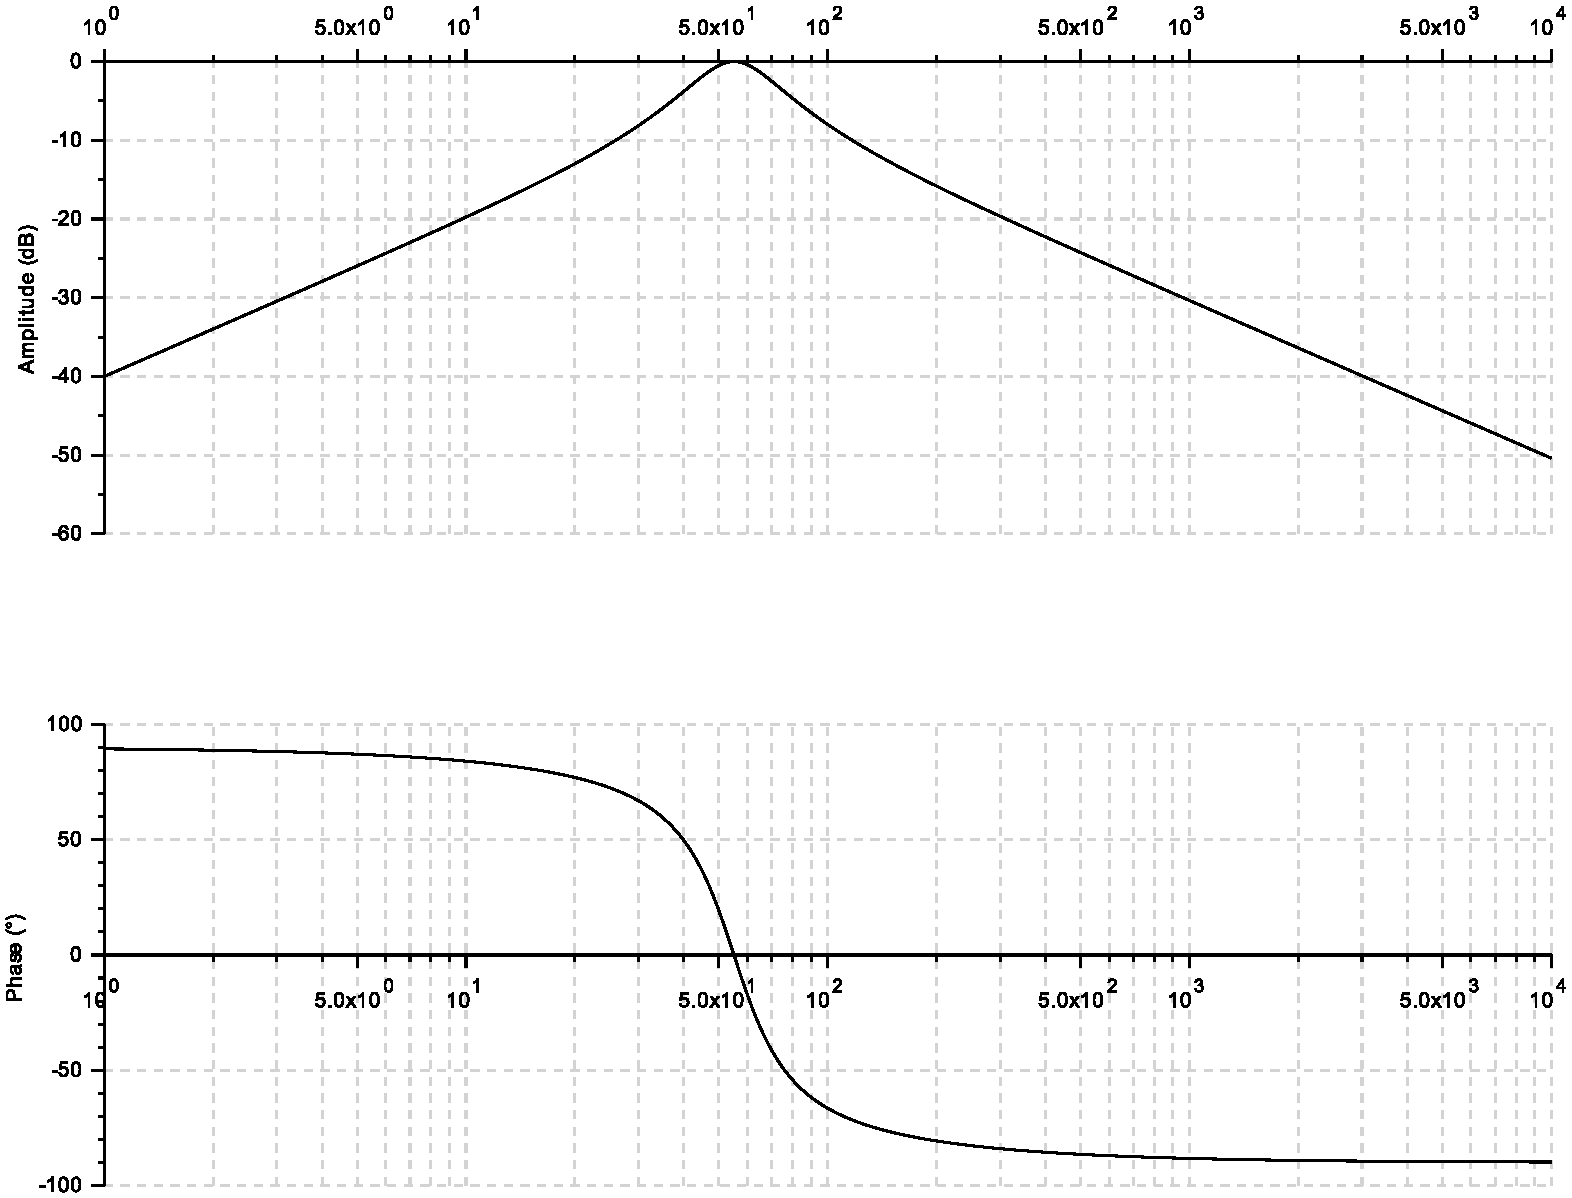
\includegraphics[width=0.9\linewidth]{img/bode2_cor}
\end{center}

\cor

Le diagramme de Bode qui correspond à la fonction de transfert $H(p)$ est la solution \textbf{a}, car la \textbf{b} correspond à la fonction $H_1(p).H_2(p)$. De plus, $\frac{1}{100}$ est faible de $1$, donc cela explique que le tracé ressemble à celui de $H_1(p)$.

\cor

La valeur finale est $1$, donc $K=1$.

D'après la lecture, on trouve un dépassement de $\frac{1,48-1}{1}=0,48$, ce qui donne sur le premier graphe $\xi=0,2$.

La pseudo-période est $T=1,8-0,6=1,2s$, donc d'après le second graphe $\omega_0=5,3rad.s^{-1}$.

\cor

\begin{center}
 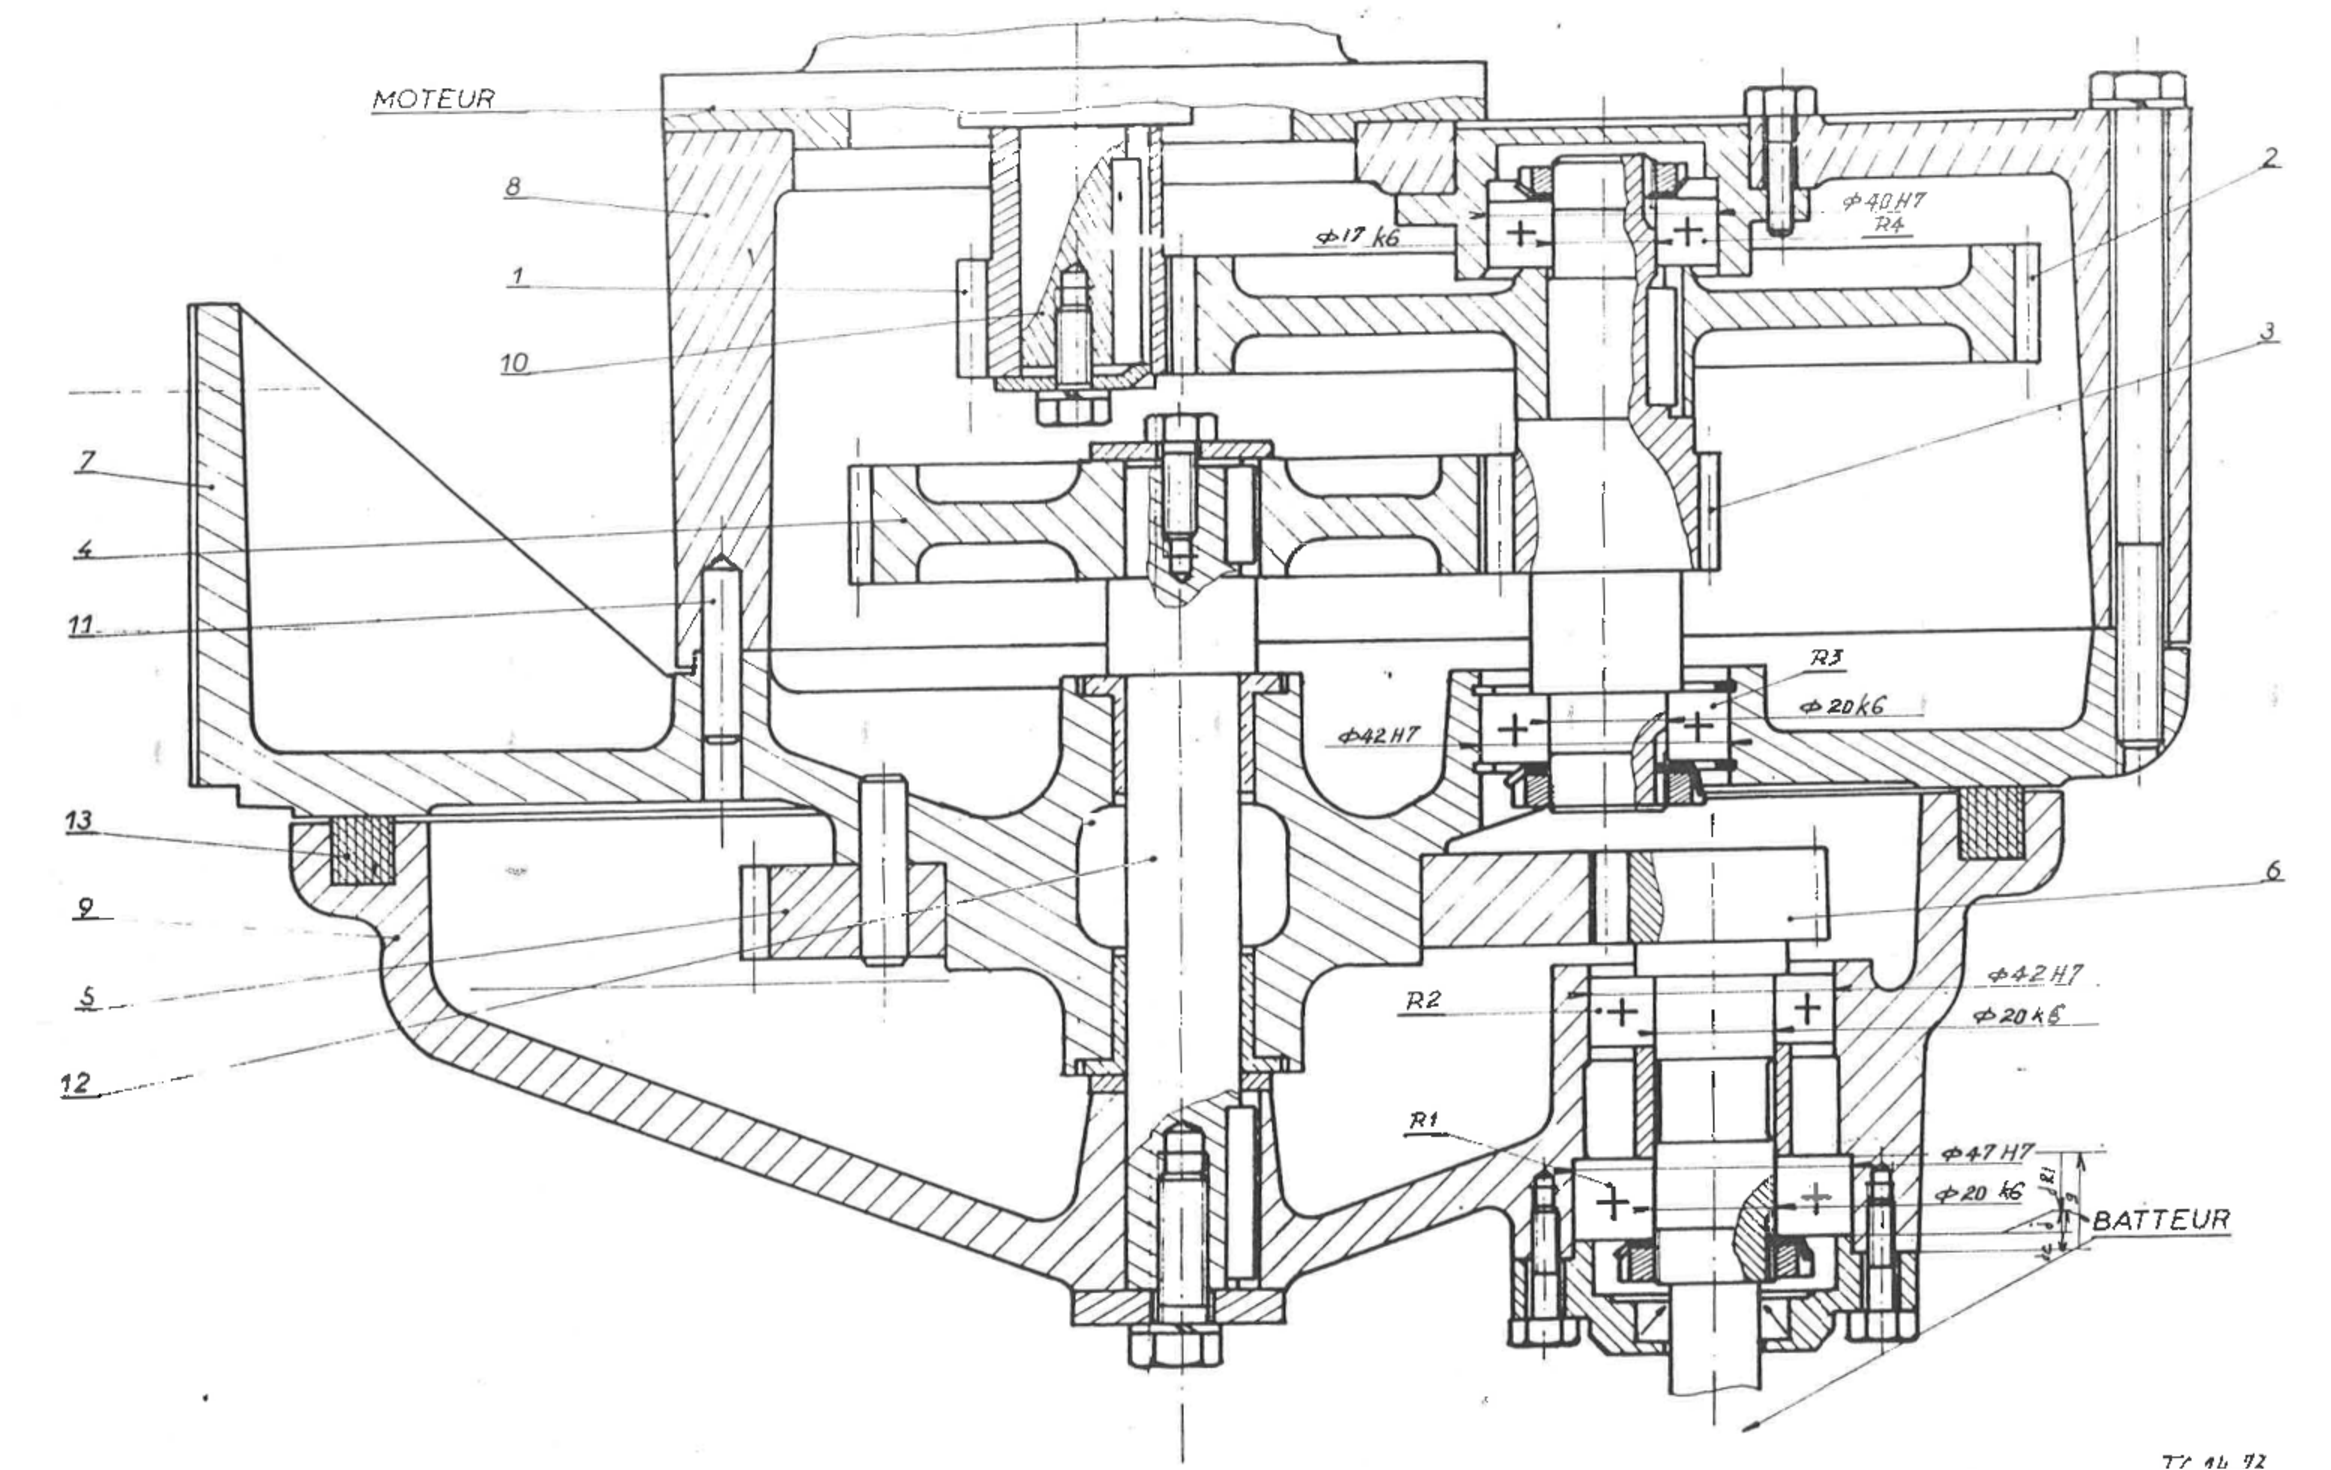
\includegraphics[width=0.9\linewidth]{img/Malaxeur}
\end{center}

\end{document}

